%==============================================================================%
%                               RAPPORT DE STAGE                               %
%==============================================================================%
% Auth: Rémi CHASSAGNOL                                                        %
% Desc: Rapport de stage de deuxième année à l'école l'ISIMA.                  %
%==============================================================================%

% Settings ---------------------------------------------------------------- {{{
\documentclass[a4paper]{article}

\usepackage[utf8]{inputenc}
\usepackage[T1]{fontenc}
\usepackage{textcomp}
\usepackage{url}
\usepackage{hyperref}
\usepackage[top=2.5cm,bottom=2.5cm,right=2cm,left=3cm]{geometry}
\usepackage[french]{babel}
\usepackage[backend=biber,style=ieee]{biblatex}
\usepackage{glossaries}
%\usepackage{titletoc}% http://ctan.org/pkg/titletoc
\usepackage{qtree}
\usepackage{color}
\usepackage{setspace}
\usepackage{graphicx}
\usepackage{geometry}
\usepackage{titlesec}
\usepackage{chngcntr}
\usepackage{pgfgantt}
\usepackage{listings}
\usepackage{minted}
\usepackage{caption}
\counterwithin*{section}{part}

% separate table of content and table of appendix
\usepackage{scrwfile}
\TOCclone[Table des annexes]{toc}{atoc}
\newcommand\StartAppendixEntries{}
\AfterTOCHead[toc]{%
  \renewcommand\StartAppendixEntries{\value{tocdepth}=-10000\relax}%
}
\AfterTOCHead[atoc]{%
  \edef\maintocdepth{\the\value{tocdepth}}%
  \value{tocdepth}=-10000\relax%
  \renewcommand\StartAppendixEntries{\value{tocdepth}=\maintocdepth\relax}%
}
\newcommand*\appendixwithtoc{%
  \clearpage
  \appendix
  \addtocontents{toc}{\protect\StartAppendixEntries}
  \listofatoc
}
%
\usepackage{blindtext}

\addbibresource{refs.bib}

%===========style & geometry===========
%\lstset{style=mystyle}

 \geometry{
 a4paper,
  left=30mm,
  right=20mm,
  top=25mm,
  bottom=25mm,
 }

 \titleformat*{\section}{\LARGE\bfseries}
 \titleformat*{\subsection}{\Large\bfseries}

%================infos=================
\pagenumbering{gobble}
\begin{titlepage}

\title{Création d'un outil d'intégration continue}
\author{CHASSAGNOL Rémi}
\date{\today}
\end{titlepage}
%}}}
% Glossaire --------------------------------------------------------------- {{{
\makeglossaries
\newglossaryentry{fixture}
{
    name=fixture,
    description={todo}
}

\newglossaryentry{semaphore}
{
    name=sémaphore,
    description={todo}
}

\newglossaryentry{smodg}
{
    name=sous module git,
    description={biblithèques qui on leur propre répertoire distant, elles sont
    stockées dans un projet à part sur Gitlab.}
}

\newglossaryentry{pic}
{
    name=PIC,
    description={(Peripheral Interface Controller) famille de microcontrôleurs
    de l'entreprise Microship.}
}

\newglossaryentry{protoserie}
{
    name=protocole série,
    description={protocole dont les éléments d'informations se succèdent sur une
    seule voie entre deux points.}
}

\newglossaryentry{halfduplex}
{
    name=halfduplex,
    description={deux éméteurs ne transmettent jamais des données en même
    temps.}
}

\newglossaryentry{fullduplex}
{
    name=fullduplex,
    description={tous les éléments peuvent parler en même temps.}
}

\newglossaryentry{des}
{
    name=DES,
    description={(Data Encryption Standard) algorithme de chiffrement
    symétrique.}
}
%}}}

%------------------------------------------------------------------------------%
%                                   Document                                   %
%------------------------------------------------------------------------------%

\pagestyle{empty}
\begin{document}

% Title page -------------------------------------------------------------- {{{
\begin{titlepage}
  \hspace{\fill}
  \begin{figure}[!htb]
     \begin{minipage}{0.50\textwidth}
       \centering
       
\includegraphics[scale=0.8]{./img/logo_isima_inp.jpeg}
     \end{minipage}\hfill
     \begin{minipage}{0.50\textwidth}
       \centering
       
\includegraphics[scale=0.4]{./img/logo-ck.png}%
     \end{minipage}
  \end{figure}
  \begin{center}
    \vspace*{1cm}

    \par\noindent\rule{\textwidth}{0.5pt}
    \Huge
    \textbf{Création d'un outil d'intégration continue}
    \par\noindent\rule{\textwidth}{0.5pt}

    \vspace{0.2cm}
    \LARGE
    Rapport d'élève ingénieur\\
    Stage de $2^{ème}$ année\\
    Filière F2 : Génie Logiciel et Systèmes Informatiques

    \vspace{1.5cm}

    \large
    Présenté par : \textbf{Rémi CHASSAGNOL}

    \vfill

    \vspace{0.5cm}
  \end{center}


  \large
  \noindent
  Responsable ISIMA : Loïc YON \hfill \textbf{Soutenance: 30/08/2023}\\
  Responsable entreprise : Ludovic DESCOUT \hfill \textbf{Durée du stage: 5 mois}\\~\\
  \raggedright
  \begin{center}
  Campus des Cézeaux. 1 rue de la Chébarde. TSA 60125. 63178 Aubière CEDEX\\
  \end{center}
\end{titlepage}

\clearpage{}

%---------------------------------------------------------------------------}}}
% Table of Content -------------------------------------------------------- {{{
\pagenumbering{arabic}
\thispagestyle{empty}
\tableofcontents
\clearpage{}

%---------------------------------------------------------------------------}}}
% Remerciements ------------------------------------------------------------{{{
\section*{Remerciements}
\thispagestyle{empty}
\addcontentsline{toc}{section}{Remerciements}

\doublespacing

Les remerciements !!

\onehalfspacing

\clearpage{}

%---------------------------------------------------------------------------}}}
% Table des figures --------------------------------------------------------{{{
\listoffigures
\clearpage{}

%---------------------------------------------------------------------------}}}
% Résumé & Abstract --------------------------------------------------------{{{
%\setcounter{secnumdepth}{3}
\section*{Résumé}
\addcontentsline{toc}{section}{Résumé}

Le super résumer !
\\~\\

\noindent
Mots-clés : \textbf{C/C++}, \textbf{intégration continue}, \textbf{tests},
\textbf{systèmes embarqués}, \textbf{émulation}

\section*{Abstract}
\addcontentsline{toc}{section}{Abstract}

the amazing abstract
\\~\\

\noindent
Keywords : \textbf{C/C++}, \textbf{continuous integration}, \textbf{testing},
\textbf{embeded system}, \textbf{emulation}

\clearpage{}

%---------------------------------------------------------------------------}}}
% Introduction -------------------------------------------------------------{{{
\pagestyle{plain}
\setcounter{page}{1}
\clearpage
\section*{Introduction}
\addcontentsline{toc}{section}{Introduction}

Introduction

TODO: la partie sur la branche C principale très détailler puis on parlera de ce
qui a été fait coté évent et Qt (qui suit globalement le même principe).

plan !

\clearpage{}

%---------------------------------------------------------------------------}}}

%------------------------------------------------------------------------------%
%                                     Plan                                     %
%------------------------------------------------------------------------------%

% Contexte du projet *******************************************************{{{
\part{Contexte du projet}

\section{CKsquare}%{{{

CKsquare est une entreprise d'ingénierie, d'étude et de conseil spécialisée dans
la conception de systèmes de paiement automatisés. La société, au départ nommée
cbsquare, a été créée en 2003 par Emmanuel Bertrand et compte aujourd'hui plus
de 30 employés. Au départ, l'entreprise se tourne vers le secteur des stations
de lavage auto en créant une gamme de distributeurs de jetons. Par la suite,
elle élargie sa collection de produits articulés autour de la monétique et se
lance dans la conception de ses propres cartes électroniques.

L'entreprise conçoit des bornes principalement pour les stations de lavage auto
ainsi que les laveries mais s'intéresse aussi à d'autres marchés comme
l'hôtellerie. Un projet de casiers automatisés, qui a été présenté sur TF1, est
aussi en train de se mettre en place. Ce nouveau projet est innovent et
écologique, car il privilégiera les producteurs locaux et évitera les voyages en
voiture pour se rendre dans les grandes surfaces. Ce projet permettra à
l'entreprise de faire face au déclin des stations de lavage auto auxquelles on
impose des restrictions à cause des sécheresses de plus en plus fréquentes.
Aujourd'hui, plus de 40000 stations de lavage auto sont équipées de bornes
CKsquare. On peut voir sur la figure \ref{bornes-intro} un exemple de produits
conçues par l'entreprise.

% [bornes] {{{
\begin{figure}[h!]
  \begin{center}
  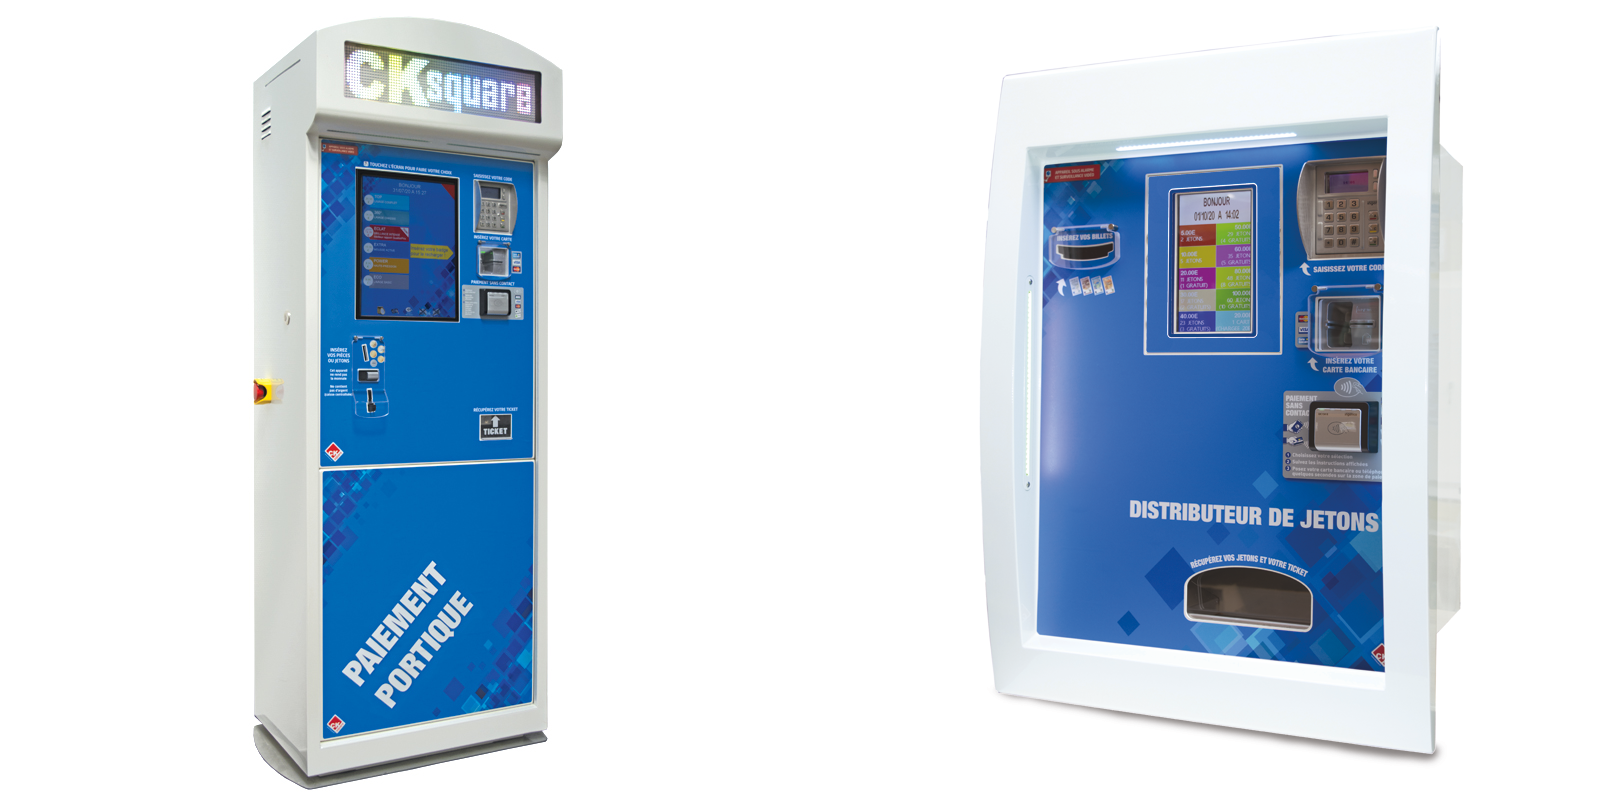
\includegraphics[scale=0.2]{./img/bornes.png}
  \caption{Produits CKsquare}
    \label{bornes-intro}
  \end{center}
\end{figure}
%}}}

CKsquare fait partie du groupe le Petit Poucet (LPP) composé de cinq sociétés
qui travaillent en collaboration. Parmi ces entreprises, on compte la société
M-Innov qui se charge de la conception et de l'installation des bornes et
systèmes monétiques pour les aires de services, campings, parking ou hôtels. La
société Mecasystem International, elle, se charge de la tôlerie et de la
mécanique pour les bornes CKsquare et M-Innov. La société Ehrse, née au sein
même de CKsquare, se charge des tests, du prés-montage et du câblage des cartes
électroniques. Enfin, il y a la société Logawin, société fille de CKsquare qui
est une entreprise de développement informatique. La société Logawin est
composée de deux pôles, Logawin France basé à Clermont-Ferrand et Logawin
Tunisie basé à Tunis. Ces cinq sociétés travaillent en coopération ce qui permet
au groupe CKsquare d'avoir la maitrise de la conception et de la fabrication de
tous les composants des produits. On peut voir sur la figure \ref{lpp-logos} les
logos des sociétés citées précédemment.

\clearpage

% [logos LPP] {{{
\begin{figure}[h!]
  \begin{center}
  
\includegraphics[scale=0.4]{./img/lpp-logos.png}
  \caption{Logos des membres du groupe LPP}
    \label{lpp-logos}
  \end{center}
\end{figure}
%}}}

L'objectif de la société CKsquare est de pouvoir fournir des produits
configurables et adaptables aux besoins des différents clients. C'est pour cela
que les bornes possèdent beaucoup d'options et que l'entreprise entretient un
savoir faire quant à la gestion de la plupart des systèmes de paiements
disponibles sur le marché. De plus, une équipe SAV reste à l'écoute du besoin
des clients ce qui permet à l'entreprise de concevoir des solutions encore plus
spécifiques et personnalisées.

Un des gros atouts de la société est son savoir faire concernant l'utilisation
des cartes électroniques. En effet, presque toutes bornes CKsquare sont équipées
de cartes électroniques beaucoup plus fiables et moins énergivores que des PC.
Cependant, ces cartes doivent assurer beaucoup de fonctionnalités et gérer un
grand nombre de composants ce qui pose de gros problèmes en terme d'optimisation
du stockage. En plus, la gestion de systèmes de paiements bancaires implique
encore plus de contraintes. Par exemple, la loi finance de 2016 (appliquée en
2018) a imposer la collection et la sauvegarde sécurisée des historiques de
paiement.
%}}}
\section{Travail demandé}%{{{

L'objectif du stage est de réaliser un outil servant à faire de l'intégration
continue pour valider les fichiers de la partie commune du code utilisé sur les
bornes. L'outil doit permettre l'écriture de tests pour valider le code et doit
pouvoir être automatisé dans une pipeline Gitlab. L'intérêt pour l'entreprise
est de pouvoir détecter un maximum de problèmes le plus tôt possible et de
manière automatique pour ne pas envoyer du code non fonctionnel en production.

L'outil sera utilisé pour tester du code normalement exécuté sur du matériel
embarqué, il faudra donc un moyen de tester des fonctions qui interagissent avec
le matériel électronique. Pour ce faire, il faudra simuler les interactions avec
le matériel en créant des fonctions et des structures de données qui réagiront
comme les composants électroniques. Par exemple, si une fonction doit modifier
un registre sur une carte, il faut pouvoir émuler le registre pour vérifier que
les bonnes modifications ont été apportées dessus. De plus, les composants
électroniques sont interfacés avec différents protocoles. Il faudra donc
comprendre le fonctionnent de ces protocoles ainsi que leur implémentation par
l'entreprise pour pouvoir simuler une communication réaliste entre la carte et
les composants.

Étant donné que les tests seront exécutés dans une pipeline (donc dans un
docker), il faudra s'assurer que le code puisse compiler sous Linux. Ici, on ne
pourra pas utiliser MPLAB et les compilateurs utilisés par l'entreprise à cause
de la simulation. Le compilateur utilisé sera gcc et une partie des
bibliothèques de Microship seront modifiées pour arriver à générer un
exécutable.

% validé
Le résultat final doit être un outil qui doit pouvoir être facilement
réutilisable et adaptable. La documentation et la structure du code doit pouvoir
permettre d'aisément modifier ou copier les différents éléments. Par exemple, il
faudra que tous les composants simulés aient la même structure et que cette
structure soit suffisamment simple et générique pour pouvoir être copiée pour la
création d'un nouveau composant.

% validé
À noter que l'objectif du projet n'est pas d'écrire des tests.  Des tests ont
été écrits durant le projet mais ces derniers ont pour objectif de valider le
bon fonctionnement des composants simulés et non celui du code de la société.
Par contre, il faudra fournir une documentation complète décrivant comment
tester les programmes. Cette documentation devra présenter le framework de test
et décrire le fonctionnement des composants simulés ainsi que leur utilisation.
%}}}
\section{Environnement et outils à disposition}%{{{

Concernant les conditions de travail durant le stage il faut noter que ce projet
se réalisait seul. Cependant, les développeurs de CKsquare étaient présents pour
répondre aux différentes questions, guider le projet ou pour faire les choix
importants.

Le projet a été démaré de zéro, aucun projet de test similaire n'avait été
amorcé auparavant. Le travail a été réalisé entièrement en présentiel. De plus,
les stagiaires étaient tous conviés aux réunions qui permettent de faire le
point au niveau des équipes de développement. Dans ces réunion chaque
développeur parle pendant deux minutes du travail qu'il a réalisé et de ce qu'il
compte faire ensuite.

Quant au matériel, un bureau avec un PC sous Ubuntu a été mis à disposition. La
session sur le PC possédait les privilèges administrateur pour faciliter
l'installation des différents logiciels utilisés pour le développement
(compilateur, éditeur de texte, doxygen, ...). De plus, il a été fourni une
boite mail ainsi qu'un compte Gitlab. Un projet Gitlab a aussi été créé pour
permettre de tester les frameworks de test. Il a aussi servit à stocker les
notes prise sur le projet ainsi que la documentation. Enfin, la documentation
des différents éléments comme les protocoles (Cctalk, Mdb) était disponible à la
demande.
%}}}
\clearpage
%***************************************************************************}}}
% Réalisation et conception ************************************************{{{
\part{Réalisation et conception}

\section{Choix du framework de test}%{{{

Le but du projet est de concevoir un outil permettant de tester du code, la
première tâche à donc été de choisir un framework de test. Le framework de test
constitue la base de l'outil, c'est donc un choix assez important. Dans cette
partie nous traiterons de la procédure qui a été utilisée pour trouver et
comparer des frameworks et des bibliothèques de test.

\subsection{Les critères de comparaison}%{{{

Étant donné le fait que le langage C est très utilisé, il y a beaucoup de choix
quand aux différentes bibliothèques de test utilisables. Le premier travail a
été de comparer bibliothèques et frameworks de tests existants. Une liste des
frameworks disponibles sur Wikipédia \cite{enwikiframeworks} a permis de prendre
connaissance des frameworks disponibles pour ensuite pouvoir faire plus de
recherches. Ce travail de recherche à permis de faire un prés tri et d'éliminer
les framework incomplets ou trop peu utilisés. Une fois la liste des meilleurs
frameworks terminée, il a fallut trouver des critères pour comparer les
frameworks. \\

Tout d'abord, l'équipe de développement souhaitait pouvoir tester à la fois du
code \textbf{C} et du code \textbf{C++} pour certaines parties développées par
l'équipe \textbf{Qt}. Ce critère était optionnel mais apprécié. À noter que
lorsque l'on parle de pouvoir tester du code C++, cela ne prend pas seulement en
compte le fait de pouvoir exécuter des fonctions basiques puisque c'est possible
avec tous les frameworks C étant donné la compatibilité entre le C et le C++.
Pour pouvoir tester du code C++, il faut aussi que le framework soit capable
d'interagir avec les structures de donnés fournis par la bibliothèque standard
de C++ ou encore de pouvoir traiter des exceptions. Étant donné ce critère,
l'idée d'utiliser un framework écrit en C++ a été envisagé.

Un autre critère concerne la modernité et la facilité d'utilisation du
framework. Cela peut sembler anodin mais l'écriture des tests est une tâche
aussi longue que le développement. Pour ne pas perdre de temps, il est
préférable que les tests soient le plus simple possible à mettre en place. De
plus, les tests peuvent aussi servir de documentation, c'est donc un avantage
non négligeable que d'avoir un framework qui permette d'écrire des tests
simples, lisibles et compréhensibles. Enfin, ce critère impacte aussi le temps
de conception de l'outil de test car le fait d'utiliser un framework trop
complexe aurait nécessité la conception de fonctions et macros (pour réduire la
complexité) et rallongé le temps d'écriture de la documentation. À noter que
pour valider ce critère, la documentation des différents outils a aussi été
étudiée, les frameworks devaient donc fournir une documentation suffisamment
claire et précise permettant d'utiliser facilement toutes les fonctionnalités
proposées.

% TODO: reformuler
Le critère le plus important est celui du statut du développement du framework.
En effet, lorsque l'on souhaite utiliser un outil, une question importante à se
poser est de savoir ce que l'on peut faire en cas de problème. Ici, il a fallut
regarder la taille, la popularité et l'age des projets. En effet, plus un projet
est populaire plus il sera facile de trouver de l'aide en cas de problème. De
plus, les projet important ont souvent beaucoup plus de collaborateurs ce qui
peut accélérer la corrections des bugs ou la vitesse de réponse au issue. Enfin
la dates de dernières mis à jours ont aussi été répertoriées car là aussi, il
est beaucoup plus simple de résoudre les problèmes sur un projet qui est encore
activement maintenu.

% TODO: mal dit
D'autres critères ont permis de démarquer les frameworks comme par exemple le
fait que les frameworks fournissent des fonctionnalités supplémentaires comme
l'export des résultats des tests dans différents format comme TAP ou XML (utile
pour faire des rapports) ou encore des générateur de nombres pseudo aléatoires
pour faire des tests avec des entrée aléatoires, \dots Une autre fonctionnalité
intéressante est que les frameworks exécutent les tests dans des threads séparer
ce qui permet de tester des signaux ou encore de ne pas stopper tous les tests à
cause d'une sortie erreur. Le fait que les frameworks utilisent beaucoup de
macros à aussi été pris en compte car bien que ces dernières permettent de
rendre le code beaucoup plus simple, elles peuvent aussi être source de
problèmes (elles ont parfois un comportement non souhaité et elles sont très
compliqué à déboguer). Le frameworks qui a été choisi possède ce défaut et nous
verrons les problème que cela pose lorsque nous détaillerons ce framework.
%}}}
\subsection{Les frameworks}%{{{

Dans cette section, nous allons faire une revue de tous les frameworks de tests
étudiés pendant le début du stage. Une fois ceci fait, nous présenterons le
choix final.

\subsubsection*{Check}

Le premier framework de la liste est Check, il propose un interface simple pour
l'écriture des tests, cependant, toute la mise en place des suites de tests est
plus complexe mais peut être changée facilement. Check permet d'exécuter les
tests dans des zones mémoires séparées ce qui permet de ne pas s'arrêter lors de
l'émission d'un signal comme SIGSEV. La bibliothèque Check est disponible avec
un paquet aptitude, ce qui le rend simple à installer. C'est aussi une bonne
preuve de la popularité de cette bibliothèque. Check est assez complet et donne
un rapport clair et facile à utiliser après l'exécution des tests. Le framework
permet de construire une structure de tests classique où l'on groupe les tests
dans des suites. Par contre, Check n'est pas compatible avec le C++.

Pour présenter les framework aux développeurs de la société, des exemples de
codes ont été présentés pour permettre d'avoir une idée de comment le framework
s'utilise. Sur le listing \ref{check-example} de l'annexe
\ref{appendix:frameworks-code} on peut voir un exemple d'utilisation de Check.

\subsubsection*{CUnit}

Le second framework est CUnit, il est aussi disponible avec un paquet aptitude
cependant. Le frameworks est assez complet et fourni beaucoup de fonctions
d'assertion. CUnit permet de construire la même structure de tests que Check, et
utilise des pointeurs de fonctions pour construire les suites. Pour chaque suite
de tests, on peut fournir deux fonctions qui seront exécutées avant et après les
tests pour permettre d'initialiser l'environnement de tests (ces fonctions sont
généralement appelées \textbf{setup} et \textbf{teardown}). Ce framework ne sera
pas compatible avec C++. Le framework CCPUnit est similaire à CUnit et permet
aussi de tester du code C, cependant, il est nécessaire d'utiliser des classes
C++ ce qui rend les tests plus complexes à mettre en place.

On peut voir sur le listing \ref{cunit-example} de l'annexe
\ref{appendix:frameworks-code} un extrait de code utilisant CUnit.

\subsubsection*{Criterion}

Le framework suivant est Criterion qui est assez récent et aussi disponible avec
un paquet aptitude. Il propose une interface très simple pour écrire des tests
et des suites de tests. On peut facilement ajouter les fonctions de setup et
teardown (pour les tests et les suites de tests) et les tests peuvent êtres
paramétrés. Comme Check, les tests sont exécutés dans des zones mémoires
séparées. On peut aussi facilement tester si un signal (comme SIGSEV) est émis
ou pas. De plus, le framework propose beaucoup de macros permettant de faire des
assertions non seulement sur les types primitifs, mais aussi sur les tableaux.
Enfin, Criterion possède aussi une interface C++.

À noter tout de même que la simplicité de l'interface de Criterion vient du fait
que le frameworks utilise beaucoup les macros ce qui peut poser problème.

On peut voir sur le listing \ref{criterion-example} de l'annexe
\ref{appendix:frameworks-code} un example de tests écrits avec Criterion.

\subsubsection*{Minunit}

Minunit est la plus simple des bibliothèques de tests trouvée. Elle ne se
compose que d'un fichier d'entête. L'interface proposée est très simple mais
très basique, elle permet seulement l'écriture de tests et de suites de tests.
Cette bibliothèque est une collections de macros qui pourraient être utilisées
pour créer un framework de test plus complet. La bibliothèque fourni aussi
quelque fonctions d'assertion.

On peut voir sur le listing \ref{minunit-example} de l'annexe
\ref{appendix:frameworks-code} un exemple d'utilisation de Minunit.

\subsubsection*{Munit}

Munit propose une interface plus complexe car cela nécessite d'utiliser des
tableaux et des structures. Pour les tests, les fonctions de tests sont très
simple à écrire et il y a la possibilités d'avoir différents types de retours.
Pour chaque test, on peut associer les fonctions de setup et de teardown. Les
tests peuvent aussi être paramétrés. Le framework propose aussi une interface en
ligne de commande, il est donc possible de donner des paramètres au programme
pour choisir quels tests sont exécutés. Il est aussi possible de construire une
structure de test plus complexe cas on peut avoir des suites de suites de tests.
Le framework propose aussi des fonctions de génération de nombres aléatoires.

On peut voir sur le listing \ref{munit-example} de l'annexe
\ref{appendix:frameworks-code} comment s'utilise Munit.

\subsubsection*{Unity}

Framework de test spécialisé pour les systèmes embarqué, léger et simple. Il ne
permet pas de construire une structure de tests très complexe (seulement de
simple tests) mais possède beaucoup de fonctions d'assertion. En terme
d'interface, le framework propose une collection de macros simples et lisibles.
Le framework fourni aussi un script pour faciliter la mise en place des tests
(en revanche ce script est assez mauvais car il ne génère un runner que pour une
seule suite).

Le framework possède beaucoup de fonctions d'assertions mais il ne possède pas
beaucoup plus de fonctionnalités. Il ne sera pas utilisable pour tester du code
qui utilise des fonctionnalités propres à c++ comme les exceptions par exemple.

On peut voir sur le listing \ref{unity-example} de l'annexe
\ref{appendix:frameworks-code} un exemple de test utilisant Unity.

\subsubsection*{Tau}

Très léger, le framework ne se compose que de fichiers d'entête. Il permet de
construire une structure de tests avec des tests et des suites de tests. Les
tests sont écrits en utilisant des macros, ce qui rend l'interface très simple.
Tau permet facilement d'avoir plusieurs fichiers de tests en générant son propre
main. Par contre, il ne permettra pas de tester les exceptions en C++.

On peut voir sur le listing \ref{tau-example} de l'annexe
\ref{appendix:frameworks-code} un extrait de code utilisant Tau.
%}}}
\subsection{Le choix final}%{{{

Le choix final s'est porté sur Criterion car le framework possède beaucoup
d'avantage. Tout d'abord, il est le seul à être complètement compatible avec le
C++ et ce, sans proposer une interface nécessitant la mise en place de classe
comme ce que l'on pourrais voir avec CPPUnit. De plus, ce framework est très
simple d'utilisation, il permet d'écrire des tests clairs facilement et
rapidement. Il propose aussi beaucoup de fonctionnalités comme la possibilité de
générer des logs, les tests paramétrés, les théories (tests des vecteurs
d'entrées et de sorties) et possède aussi une interface en ligne de commande
permettant de passer des options en paramètres du programme.

Par contre, la simplicité d'utilisation de ce framework cache une grande
complexité au niveau de son implémentation. Le framework a posé quelques
problèmes mineurs dans la suite du projet. Tout d'abord, la simulation des
composant nécessite l'appel de fonctions d'initialisation au préalable et cela
aurait été pratique de le faire dans la fonction \verb|main|. Comme
expliqué dans les parties précédentes, le framework génère son propre point
d'entré, cependant il est possible d'écrire la fonction \verb|main| à la
main si besoin. Le problème est que pour une raison inconnue, cela n'a pas
marché lors des essais au début du projet (d'après le message d'erreur, le
problème venait des threads). Ce n'est pas un problème grave car Criterion
propose beaucoup d'outils qui permettent de mettre en place des solutions
alternatives mais c'est tout de même un point important à noter. De plus, le
fait que le framework utilise beaucoup de macros pose parfois problème car ces
dernière peuvent avoir des comportements indésirables. Par exemple, il peut
arriver qu'un test basique d'égalité avec la fonction d'assertion principale ne
compile plus lorsque l'on échange les expressions de par et d'autre de
l'opérateur \verb|==|. Les macros peuvent être très utiles et très
puissantes, elles permettent ici de rendre le code beaucoup plus lisible,
cependant, il faut noter que les macros trop complexe sont très difficiles à
écrire et à déboguer.

Le framework choisit possède donc beaucoup de qualité mais aussi quelques
défauts. Au final, bien que ce framework ne soit pas parfait, il remplit
bien son rôle et il propose beaucoup de fonctionnalités très utiles pour
écrire les tests. De plus, il faut noter que ce framework est assez récent, il
est donc normal qu'il y ai encore des défaut qui seront certainement corrigés
au fil des années de développement.
%}}}
%}}}
\section{Organisation d'un projet CKsquare}%{{{

L'outil créé pendant ce stage a été testé sur un projet de l'entreprise. Cela a
permis dans un premier temps de pouvoir voir et comprendre comment le code à
tester fonctionnait puis ensuite cela à permis de vérifier la bonne intégration de
l'outil dans le projet. Dans cette partie, nous détaillerons comment sont
organisés les projets de CKsquare. Cela permettra une meilleur compréhension des
choix qui ont été fait par la suite.

\subsection{Organisation des fichiers}
\label{orgaprojck}

TODO: arborescence des fichier pour le projet global et pour \verb|dev_pic|

Dans cette partie, nous allons détailler comment sont organisés les fichiers
dans un projet CKsquare puis nous traiterons le fonctionnement du code dans la
partie suivante. On rappel que ce projet d'intégration continue ne concerne que
la partie du code qui est commune à tous les projets. Elles fait parties des
bibliothèques ajoutés aux projets sous la forme de \gls{smodg}. \\

Pour pouvoir penser le fonctionnement de l'outil de test à créer pendant ce
stage, il était important de comprendre le fonctionnement général du projet.
Avant de s'intéresser au fonctionnement, il faut comprendre comment le code est
organisé. Cela permet deux choses, premièrement, cela permet de ne pas se perdre
et de pouvoir facilement retrouver les fichiers. Pour comprendre le
fonctionnement du code, il est important d'avoir un plan de l'organisation.
Deuxièmement, il est aussi très important de comprendre comment s'est organisée
l'entreprise pour pouvoir structurer le code de l'outil créé. En
effet, l'organisation du projet de test doit suivre les principes de CKsquare
pour rendre l'outil facile à utiliser et à maintenir pour les développeurs de
l'entreprise.

%TODO: expliquer brièvement le projet myosis et pk il a été choisi

Chaque projet comporte une partie locale dans laquelle, tous les noms de
fichiers commencent par un \textbf{l}. Dans cette partie, on retrouve trois
fichiers principaux. Tout d'abord, il y a le fichier \verb|linit.c| qui permet
d'initialiser le projet. Ensuite, il y a les fichiers \verb|lmain.c| et
\verb|lloop.c| qui permettent de gérer la fonction \verb|main| et la boucle
principale du projet. Le projet local contient aussi deux fichiers très
importants car ils permettent de configurer le projet. Ces fichiers se nomment
\verb|config.h| et \verb|config_hw_default.h|. Ce sont des fichiers d'entête à
l'intérieur desquels sont définis des constantes préprocesseur. Les projet
CKsquare fonctionnent beaucoup sur le principe de la compilation conditionnelle.
Les constantes préprocesseurs sont gérées à la compilation pour inclure ou non
des parties du code, ce qui permet d'ajouter ou d'enlever facilement des
fonctionnalité. Lorsqu'une fonctionnalité est enlevée, elle n'est pas compilée
et le code correspondant n'apparait pas dans l'exécutable. De ce fait, il
n'impacte pas sa taille, ce qui est très intéressant du fait des limitations
quand aux capacités de stockage sur les carte. La gestion de la configuration
s'est avérée complexe du fait du grand nombre d'options qui ne sont pas toutes
documentées. Chaque projet contient aussi un répertoire \verb|CKLibs| dans
lequel se trouvent des \gls{smodg}. Sur le projet d'étude qui a permis la mise
en place du projet de test, il y avait deux sous modules. Le premier sous module
se nomme \verb|commun_global| et il contient la partie du code qui est commune à
tous les projet C, C++ et python. Le second sous module est \verb|dev_pic|, ce
dernier ne concerne que la partie C qui s'exécute sur un \gls{pic}.

La partie que nous allons traiter se trouve dans le répertoire \verb|dev_pic|
(aussi appelé codes communs). Ce répertoire contient un sous répertoire
\verb|commun| qui contient la partie du code à tester. À la racine des communs,
se trouvent aussi une partie des bibliothèques des différents compilateurs.
L'entreprise CKsquare a réécrit une grande partie des bibliothèques des
\gls{pic}s pour avoir plus de maitrise quand à la gestion des différents
éléments. Ces bibliothèques ont été très utiles pour mettre en place une partie
de l'émulation des composants dans le projet de test, nous traiterons cela plus
loin dans ce rapport. Le reste des bibliothèques des microcontrôleurs a aussi
été utilisé pour compiler avec gcc, là aussi, ce sera traiter dans les
prochaines sections.

Le code commun est organisé par catégories. Le répertoire \verb|commun| de
\verb|dev_pic| contient des sous répertoires qui correspondent aux
catégories. Par exemple, on retrouve le dossier \verb|StorageDriver| qui
contient les fichiers qui gèrent le stockage ou encore le dossier
\verb|Payment| qui contient tous ce qui concerne le paiement (types de
paiement, accepteur de pièce, \dots). L'objectif est de pouvoir faire des
recherche par catégories et de garder les dépendance au plus proche des
fichiers. Par exemple, plusieurs des sous répertoires de \verb|commun|
contiennent un dossier \verb|Web| qui regroupe les dépendances web des
fichiers de chaque catégories. On peut ainsi retrouver facilement les dépendance
des fichiers.

Pour résumer, les projets CKsquare sont composés d'une partie locale, spécifique
au projet. Parmi ces fichier locaux, on retrouve le fichier responsable de
l'initialisation, le point d'entrée, la boucle principale ainsi que la
configuration du projet. Les projets incluent des bibliothèques sous la forme de
\gls{smodg} stockées dans le répertoire \verb|CKLibs|. Parmi ces
bibliothèques on retrouve le projet \verb|dev_pic| qui contient le code
commun à la partie C qui s'exécute sur les cartes électroniques de l'entreprise,
et c'est ce code que l'outil créé durant ce stage va testé. À noter qu'ici, on
ne s'intéresse qu'à l'essentiel pour permettre une explication rapide du
fonctionnement général du projet dans la partie suivante. Cependant, le projet
comporte beaucoup d'autres fichiers qui ne sont pas décrit dans ce rapport.\\

Maintenant que nous avons expliqué l'organisation générale du projet, nous
allons pouvoir traiter le fonctionnement de ce dernier.

\subsection*{Fonctionnement du projet}

Le code commun comporte deux branches, une branche principale et une branche
plus récente sur laquelle le code fonctionne avec un système d'évènement. La
branche sur l'événementiel a été traitée en deuxième partie de stage.

Sur les deux branches, le code est géré par des machines à états. Elles sont
utilisées autant du côté du C que de celui du C++. Les machines à état sont un
outil très puissant est très pratique car elles permettent d'avoir un meilleur
contrôle sur l'exécution du code et ont un fonctionnement assez intuitif. De
plus, elles peuvent permettre de rendre le code plus clair en particulier quand
il y a beaucoup de cas à traiter. Enfin, elles permettent de gérer les erreurs
simplement en évitant la duplication de code.

\subsubsection*{Branche principale}

Cette branche a été la première créée par les développeurs de la société, elle
est utilisée sur la plupart des bornes. Le principe est que chaque fichier
fournit une fonction \verb|Control| (exemple: \verb|BILLVALIDATOR_Control|). Ces
fonctions sont des machines à états qui permettent de contrôler une
fonctionnalité. Par exemple, pour un accepteur de billet, la fonction
\verb|Control| aura des états qui seront utilisés au début et qui vont permettre
de faire de l'initialisation. Ces états peuvent faire des requêtes au composant
pour récupérer sa configuration. La machine à états aura aussi un état servant à
interroger le composant durant sont exécution, pour par exemple savoir si il y a
un billet à traiter.

Les fonctions \verb|Control| sont appelées par un gestionnaire
(\verb|ControlManager|). À l'initialisation du programme, toutes les fonctions
\verb|Control| sont ajoutées dans une liste et pour chacune d'entre elles, on
précise la durée minimale entre deux appels. Ensuite, le gestionnaire est
utilisé dans la boucle principale et va appeler toutes les fonctions qui ont été
ajoutées lorsque c'est nécessaire. Par exemple, on peut ajouter la fonction de
l'accepteur de billet à l'initialisation et spécifier que cette fonction soit
appelée toutes les dix centièmes de seconde. Avec cette configuration, la
fonction sera appelée par le gestionnaire et il y aura au minimum dix centièmes
de seconde entre chaque appel.

Les fonctions \verb|Control| vont être un élément très important à tester. Ces
fonctions ont beaucoup servi lors des essais réalisé sur les fichiers pendant la
création de l'outil. Elles sont très intéressantes car elles permettent de
couvrir une grande quantifié de code et de tester la plupart des cas (pour le
code de l'outil de test). À noter cependant que les machines à états sont très
compliquées à tester puisqu'il ne faut normalement pas avoir accès aux états
dans les tests \cite{teststatemachines}. Il faut donc être capable de manipuler
l'environnement dans le code pour savoir dans quel états on se trouve et choisir
l'état dans lequel se rendre. L'utilisation d'un débogueur a grandement facilité
la mise en place des tests réalisés sur ces fonctions.

\subsubsection{Branche événementiel}
\label{brancheevent}

Cette branche a été créée pour simplifier le code, elle utilise un système mis
en place sur la partie Qt (code C++) qui intègre un système permettant de
déclencher des appels de fonctions en émettant des évènements. Le deuxième
objectif de ce système est de limiter les appels de fonctions dans la boucle
principale. En effet, sur l'autre branche, les fonctions \verb|Control| des
composants sont continuellement appelées par le \verb|Contro Manager|, ce qui
peut poser des problèmes de performance. Ici, les fonctions qui gèrent les
composants ne sont appelées que lorsqu'un évènement est émit. Par exemple,
lorsqu'une trame est envoyée, un évènement est émit pour signifier la fin de la
communication. Cela aura pour effet de déclencher l'appel de la fonction de
gestion du composants qui a envoyé la trame. Cette fonction est une machine à
états qui passera dans un état d'attente de réponse.

TODO: event\\
TODO: inspiré de qt\\
TODO: plus lisible mais plus lourd\\
TODO: normalement plus rapide comme il n'y a pas trop d'appels à toutes les
fonctions

%}}}
\section{Organisation du projet de tests}%{{{

Dans cette partie, nous allons détailler la structure du projet de test. Cette
structure s'appuie sur celle des projets de l'entreprise.

Il est important de noter que l'organisation du projet de test à changée. Au
départ, le projet de test devait être un géré à part. Ce dernier devait être
cloné dans la pipeline du code commun pour pouvoir tester les fichiers. Au
final, il a été décidé d'intégrer complètement l'outil de test dans
\verb|dev_pic|. L'organisation des tests suis les principes expliqués dans la
section \ref{orgaprojck}. De ce fait, les tests sont stocké à proximité des
fichiers testés. Sur la figure \ref{fig:integrtestcommun}, on peut voir une
représentation de l'arborescence des fichiers dans le projet commun.

% TODO: une partie de l'arborescence est normalement présenté dans la partie
% précédente

% [Intégration des tests dans le code commun] {{{
\begin{figure}[h!]
  \begin{center}
    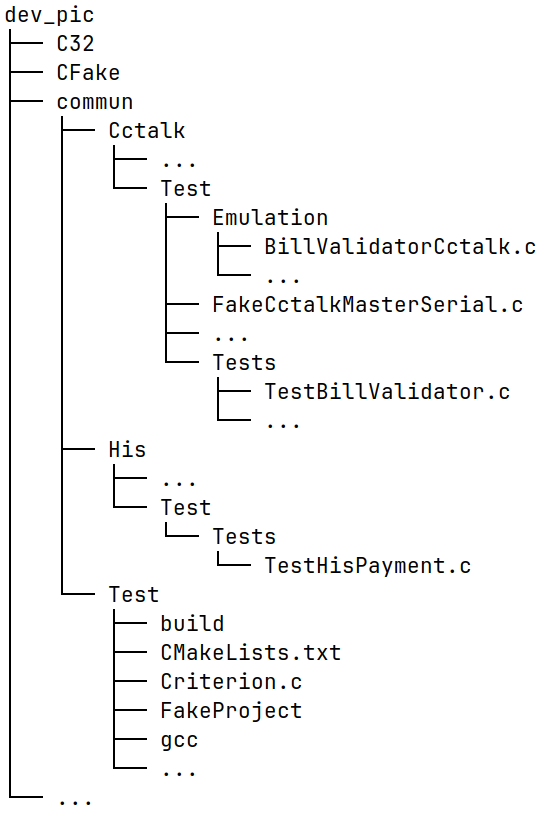
\includegraphics[scale=0.7]{./img/arborescence-commun.png}
    \caption{Intégration des tests dans le code commun}
    \label{fig:integrtestcommun}
  \end{center}
\end{figure}
%}}}

Cette arborescence montre une partie du contenu du répertoire
\verb|dev_pic/commun|. Ici, on peut voir trois des catégories qui ont été
mentionnées dans la section \ref{orgaprojck}. Il y a le dossier \verb|Cctalk|
qui contient le code qui permet de gérer le protocole Cctalk que nous aborderons
dans une prochaine partie. Le dossier \verb|His| lui contient le code qui permet
de gérer l'historique. Enfin, le répertoire \verb|Test| a été ajouté lors de
l'intégration du projet de test dans le projet commun, ce dernier contient les
fichiers généraux spécifiques aux test. À noter qu'il y a un autre répertoire
\verb|CFake| qui lui se trouve à la racine du projet, au même niveau que
\verb|commun|. Ce dernier contient la simulation des interfaces pour le
stockage. Étant donné que le stockage est un élément assez général, il a été mis
à part. Comme on peut le voir ici, tous les fichiers ayant un lien entre eux
sont stockés ensemble et il en est de même pour les tests. C'est une structure
assez atypique pour du C puisque les tests sont habituellement mis à part,
généralement dans un répertoire \verb|test| à côté du projet. Ici, les tests
sont intégrés dans code à la demande des développeurs de la société. C'est un
choix assez intéressant puisque cela permet d'avoir accès aux tests très
rapidement et de bien voir à quels éléments du code les tests sont liés.

Maintenant que nous avons définie une carte générale du projet, détaillons les
parties les plus importantes.

\subsection{Le répertoire Test principal}

Comme expliqué précédemment, ce répertoire contient des fichiers globaux
qui permettent de pouvoir compiler et exécuter les tests. Les différentes
parties sont décrites dans les sections suivantes.

\subsubsection*{Faux projet}
\label{fakeproj}

Ce fichier contient des versions modifiées des fichiers du projet local (ceux
dont le nom est préfixé d'un \verb|l|). Il contient aussi les fichiers de
configuration. Pendant la création de l'outil, il s'est avéré qu'il y avait des
dépendances entre les fichiers des communs et le projet local. Cela pose
problème car depuis la pipeline, on a pas accès aux fichiers locaux puisqu'ils
sont spécifiques aux différents projets. Une solution envisageable est le
clonage d'un projet depuis la pipeline, cependant cette méthode possède deux
gros défaut. Le premier réside dans le fait de devoir cloner un projet entier
juste pour exécuter une pipeline, cela prend du temps et des ressources. Le
deuxième défaut vient du fait que la configuration des tests n'est pas la même
que celle du projet local. En effet, dans les tests, on ne peut pas compiler
tous les fichier (car tout n'a pas été simulé et tout ne doit pas être testé) et
on utilise une configuration qui permet de pouvoir tester plusieurs
fonctionnements différents. De ce fait, il est impossible de compiler les tests
en utilisant les fichiers originaux. C'est pour ces raisons qu'il a été décidé
de récupérer seulement les fichiers nécessaire à la compilation des tests et de
les modifier si besoin.

\subsubsection*{Gcc}
\label{gcc}

Ce répertoire contient des versions modifié des fichiers du compilateur
\verb|c32| (normalement stockés dans le répertoire \verb|C32| à la racine des
communs). Là aussi, les fichiers sont modifiés pour que le code puisse compiler
avec \verb|gcc|. À noter que ce répertoire contient un fichier créé à partir de
la bibliothèque \verb|plib| qui définie toutes les variables globales
normalement utilisées par les bibliothèques carte. Tous les fichiers contenus
dans ce répertoire permettent donc de compiler le code sans avoir accès au
bibliothèques du \verb|PIC|.

\subsubsection*{Configuration de Criterion}
\label{configuration-de-criterion}

Pour que les tests incluant l'émulation de composants fonctionnent, il faut
pouvoir lancer et initialiser la simulation. Pour ce faire, on utilise un
fichier qui fourni des fonctions d'initialisation et de terminaison globales qui
peuvent être utilisées dans les test. La fonction d'initialisation permet de
créer les threads utilisé pour les horloges comme nous le verrons dans la
section \ref{simuhorologes} ainsi que d'initialiser toutes les variables
nécssaire au bon fonctionnement de la simulation. Dans la fonction de
terminaison, on termine simplement les threads des horloges. Dans ce fichier, on
peut aussi ajouer d'autre fonctions spécifiques au framework.

\subsection{Les répertoires de test secondaires}

Comme dit précédemment, les développeurs de l'entreprise souhaitaient stocker
les tests à proximité des fichiers testés. C'est pour cela que l'on a des
répertoires de test secondaires dans chaques répertoire du projet. Dans les
section suivant, nous allons décrire le contenu de ces dossiers.

\subsubsection{Les fichiers modifiés}

Certains tests nécessitent la création de versions modifies de certains des
fichiers de l'entreprise pour permettre d'isoler des fonctionnalités du
programme et faciliter les tests. Par exemple, les entrées et sorties sont
gérées pas un fichier nommé \verb|Ios.c|. Il est très compliqué de savoir si les
fonctions de ce fichier sont appelées depuis les tests or parfois, on a besoin
de tester si une action d'entré ou de sortie a été réalisée. Une version modifiée
de ce fichier a donc été créée pour les tests. Les fonctions de la version test
du fichier mettent à jour des variables globales accessibles depuis les tests
permettant ainsi de savoir si des actions d'entrée ou de sortie ont été
réalisées. Les versions test des fichiers sont compilés à la place des fichiers
originaux pour les tests. Cette solution est similaire au \textit{mocking} (au
niveau des fichier) qui est très utilisé avec les langages objets
\ref{spadini2017mock}.

\subsubsection{Les fichiers de la simulation}

Les sous-répertoires de test permettent aussi de stocker les fichiers qui
contiennent les éléments nécessaire à la simulation des composants. Par exemple,
les fichiers qui permettent de simuler les composants interfacés avec le
protocole Cctalk sont stocker dans le répertoire \verb|commun/Cctalk/Test|. Nous
traiterons ce protocole dans la section \ref{interfacecctalk}.

\subsubsection{Les tests}

Pour les tests, on ajoute encore un nouveau sous-répertoires à l'arborescence.
Chaque répertoire \verb|Test| contient un sous-dossier \verb|Tests| qui permet le
stockage des fichiers de test.

\subsection{Cmake}
\label{cmake}

Dans cette partie nous allons voir comment est compilé le projet de test. Nous
justifierons tout d'abord le choix de l'utilisation de CMake. Ensuite, nous
détaillerons l'organisation et le fonctionnement de la configuration de cet
outil.

Au début du projet, l'outil choisit pour compiler était Makefile. L'avantage de
Makefile est qu'il est assez proche du script, ce qui donne une grande
flexibilité car on défini toutes les commandes à la main. Le défaut de Makefile
est qu'il peut très vite devenir peu lisible. De plus, sur de gros projet, mettre
en place de la compilation séparée peut être très complexe, or cela était
nécessaire pour le développement du projet étant donnée le nombre de fichier à
compiler. L'outil de test à créer devait être suffisamment simple à utiliser et à
modifier, la complexité croissante du Makefile à mesure que le projet avançait a
pousser à l'utilisation de CMake.

CMake est un outil qui permet de générer un Makefile très complexe. Il permet de
mettre en place de la compilation séparée sur de gros projets automatiquement.
La configuration de CMake est assez simple et beaucoup plus lisible que celle de
Makefile. De plus, CMake propose des fonctionnalités avancées comme la gestion
automatique des bibliothèque ou encore \textbf{CTest}, qui permet d'automatiser
l'exécution de tests. Détaillons à présent la configuration de cet outil.

Le fichier de configuration de CMake est le fichier \verb|CMakeLists.txt|
(il doit avoir exactement ce nom). Il faut un ficher de configuration par sous
projet. Ici, il n'y a que le projet de tests alors ce fichier se trouve dans le
répertoire \verb|commun/Tests|.

La configuration comporte les six sections suivantes:

\begin{itemize}
  \item[$\bullet$] \textbf{configuration du projet}: cette partie contient la
    configuration minimale de CMake. Ici, on spécifie la version minimale de
    CMake requise ainsi que le nom du projet. Cette partie comprend aussi
    l'ajout du framework Criterion à l'édition des liens ainsi que des options
    pour \verb|gcc| comme l'option \verb|-g| par exemple (débogage
    avec gdb).
  \item[$\bullet$] \textbf{jeux de tests}: dans cette partie, il y a plusieurs
    listes de fichiers tests (stockées dans des variables réutilisables plus
    loin). Il y a plusieurs jeux de tests car on souhaite générer plusieurs
    exécutables. Comme dit précédemment, il y a plusieurs configurations du
    projet à tester. Chaque exécutable correspond à une fonctionnalité qui
    nécessite une configuration particulière.
  \item[$\bullet$] \textbf{projet de test}: cette partie contient la liste des
    fichiers relatifs au projet de test.
  \item[$\bullet$] \textbf{projet commun}: ici on a une liste qui contient les
    fichiers du projet \verb|dev_pic| qui sont à compilés avec tous les
    exécutables. Ce sont les fichiers dont tous les jeux de tests ont besoin.
  \item[$\bullet$] \textbf{exécutables}: dans cette partie, on génère les
    exécutables en spécifiant les bonnes listes de fichiers à compiler. De plus,
    pour chaque exécutable, on utilise une commande CMake qui permet de définir
    des constantes préprocesseur lors de la compilation (option \verb|-D|
    de gcc). Cela permet de choisir les configurations du projet pour les tests.
  \item[$\bullet$] \textbf{tests}: dans cette section, on ajoute les exécutables
    à la liste des tests. Ces tests pourront être lancé par \verb|CTest|
    après la compilation.
\end{itemize}

%TODO: conclusion cmake

%}}}
\section{Simulation des horloges}%{{{
\label{simuhorologes}

Le premier élément qui a été simulé était l'horloge principale du programme. Par
la suite, c'est l'horloge Rtc qui a été simulée en suivant le même principe que
pour l'horloge principale. Dans cette section nous allons traiter le
fonctionnement de ces composants.\\

Au début du projet, quelques tests simples ont été réalisés sur certains
fichiers, cependant, il est rapidement devenu évident que certaines fonctions
n'allaient pas pouvoir être testées à cause de l'horloge. En effet, à plusieurs
endroits dans le code, on met en place des temps d'attente et le programme est
bloqué tant que le temps d'attente n'est pas passé. L'horloge est gérée dans le
code à travers une variable globale \verb|TIMER_Centieme| et cette dernière
doit être incrémentée pour que le temps passe. Dans le cas contraire, le
programme reste bloqué.

Le problème technique que pose la simulation des horloges est qu'il faut que ces
dernières fonctionnent en même temps que le programme principale tourne.
L'implémentation la plus simple consiste à incrémenter les variables d'horloge
dans les tests à chaque fois que l'on sait qu'un temps d'attente est mis en
place. Cette solution n'était pas suffisamment pratique et réaliste. Pour ce
problème, il a été très rapidement décidé d'utiliser des threads. L'objectif
était d'incrémenter les variables des horloges dans des fonctions simples
s'exécutant dans un processus séparé en même temps que le programme principal.

Cette solution a été très simple et rapide à mettre en place étant donné que les
processus n'avaient pas besoin d'être synchronies. Au final, les deux horloges
fonctionnent sur le même principe. Pour chacun des fichiers on a une fonction
\verb|Start| qui permet de créer le thread. Cette fonction possède une
sécurité qui fait que l'on peut faire autant d'appels que l'on souhaite, le
thread n'est créé qu'une seule fois (cela rend l'utilisation plus simple dans
les tests). À noter que dans le cas du Rtc, l'horloge démarre à la date du jour.
Les fichier comportent aussi une fonction \verb|Loop| qui est la fonction
qui s'exécute dans le thread. De plus, des moyen d'interagir avec les horloges
ont étaient ajoutés. Par exemple, à certains endroits du code, on met en place
des temps d'attente relativement long. Pour éviter de bloquer le programme,
chaque fichier propose une fonction \verb|Wait| qui permet d'incrémenter le
compteur manuellement. Il est aussi possible de mettre les horloges en pause et
de les relancer. Enfin, il y a une fonction \verb|Stop| qui permet de
détruire les threads. Les fonctions \verb|Start| et \verb|Stop| sont
appelées dans les fonctions d'initialisation et de terminaison globales décrites
dans la section \ref{configuration-de-criterion}.\\

Les horloges représentaient donc une partie importante du projet car elles sont
énormément utilisées dans le code et si les compteurs ne sont pas incrémentés,
il devient impossible de tester les fonctions. La solution qui a été trouvée est
très simple et assez réaliste en plus d'être assez pratique à utiliser dans les
tests. Dans la section suivante, nous traiterons le deuxième éléments qui a été
simulé lors de la création de l'outil de test et qui propose une solution
différente de celle utilisée avec les horloges.
%}}}
\section{Simulation du stockage}%{{{

Une partie importante de l'émulation concerne le stockage et il y a plusieurs
types composants à simuler, les registres, les eeproms, et la mémoire flash.
L'émulation des périphériques de stockage est assez simple puisqu'il s'agit
juste de tableaux de caractères non signés (codés sur 8 bits sur la plupart des
machines). La partie complexe de l'émulation du stockage concerne l'interface
qui permet d'interagir avec les périphériques. Il y a deux protocoles qui sont
utilisés avec le stockage. Tout d'abord il y a le protocole I²C qui est utilisé
avec les registres et certaines eeproms. Ensuite il y a le protocole SPI qui est
utilisé avec les eeproms et les mémoires flash. La simulation de ces deux
interface a nécessité l'apprentissage des deux protocoles qui ne sont pas traité
dans les cours de la filière 2 à l'ISIMA.

TODO: mettre des images des composants (montrer l'objet au delà du code est
intéressant)

Dans cette partie nous allons voir comment a été réalisée l'émulation de
l'interface permettant d'utiliser le stockage avec les différents protocoles.

\subsection{Échec des threads}%{{{
\label{echecthread}

La première solution qui a été implémentée utilisait des \textbf{threads} de la
même façon que les horloges. L'objectif été de pouvoir simuler les composants de
sorte à ce qu'ils se comportent comme les composants réels installés sur la
carte. Pour se faire, il été souhaitable que les composants simulés soient actif
en même temps que la carte (représentée ici par le programme à tester) et c'est
pour cela que les threads ont été utilisés. Le principe était que les composants
étaient représentés par des machines à états qui bouclaient dans un état de base
jusqu'à ce que le composant soit appelé (donc jusqu'à ce que le programme
principale décide de lancer une communication en utilisant un des protocoles
cités précédemment). Une fois le composant appelé, la machine à états permettait
d'assurer la communication. Pour que les composants simulés s'exécutent en même
temps que le programme principale, ils s'exécutaient dans des threads séparés.
\\

Le problème des threads réside dans la synchronisation de ces derniers. Il y a
différentes méthodes pour synchroniser des threads. Sur ce projet, il a au
départ été utiliser des boucles infinies qui permettait de faire attendre les
threads. Par exemple, le programme principale était stoppé par une boucle pour
attendre que le les composants émulés s'exécutent et le débloque. Cette solution
a été utilisée au départ car ce genre de boucles été déjà présentes dans
l'implémentation de l'I²C. Par la suite, cette solution s'est avérée complexe
d'utilisation et peu élégante, les boucles ont donc étaient remplacées par des % todo: expliquer les sémaphores
sémaphores. Au final, la synchronisation des threads est devenue trop compliquée
et très peu fiable (l'exécution du programme ne donnait pas toujours les même
résultats). L'objectif du projet étant de concevoir un outil qui soit facilement
réutilisable, cette solution était trop complexe et donc pas adaptée. Il a donc
été décidé de ne plus les utiliser les threads même si la nouvelle solution
devait être moins pratique d'utilisation au niveau de l'écriture des tests.
%}}}
\subsection{Interface I²C}%{{{

Dans cette partie, nous allons voir le fonctionnement de l'émulation de
l'interface I²C du stockage. Nous commencerons par voir les principes du
protocole I²C puis nous détaillerons le fonctionnement de la simulation.

\subsubsection*{Le protocole I²C}

Le protocole I²C (Inter Integrated Circuit) est un \gls{protoserie}
bidirectionnel en \gls{halfduplex}. La plupart des connaissances sur l'I²C on
été trouvées sur ce document \cite{mankar2014review} et de Wikipédia
\cite{frwiki:197726464}, le reste vient des développeurs de l'entreprise. Ce
protocole fonctionne en mode maître et esclave. Par exemple, la carte
électronique est considérée comme le maître et elle pilote les périphériques qui
eux sont les esclaves. Un esclave ne prend jamais la parole, c'est au maître de
démarrer la communication et l'esclave répond lorsque c'est nécessaire. La
connexion est réalisée par l'intermédiaire de deux fils, SDA (Serial Data Line)
qui permet de transmettre les données et SCL (Serial Clock Line) qui correspond
à l'horloge, quand SCL est à 1, on envoi un bit sur SDA. Ces deux lignes sont
bidirectionnelles. Le schéma de la figure \ref{fig:schemai2c} illustre le
principe de l'I²C.

% [schéma i2c] {{{
\begin{figure}[h!]
  \begin{center}
    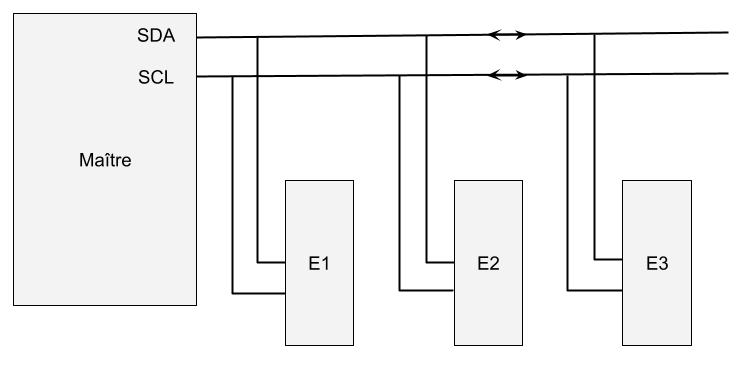
\includegraphics[scale=0.4]{./img/schema-i2c.png}
    \caption{Liaison maître/esclave (I²C)}
    \label{fig:schemai2c}
  \end{center}
\end{figure}
%}}}

Pour démarrer la communication, le maître envoi un octet que l'on appel
\textit{l'octet d'adresse}. Sur ce premier octet, les sept premiers bits
corresponde à l'adresse du destinataire (l'esclave qui est appelé par le
maître). Le dernier bit permet de spécifier le mode d'accès, s'il est à 0, le
maître va envoyer des données à l'esclave. S'il est à 1, c'est l'esclave qui
devra envoyer des données aux maître. Si on prend l'exemple du stockage, quand
ce bit est à 0, la carte va envoyer des données à écrire, sinon, la carte
souhaite lire les données écrites sur le composant. La suite de la communication
va vairée en fonction de ce qui a été demandé par la carte.

Pour résumer, ce protocole fonctionne en mode maître et esclaves avec deux
lignes, SDA qui permet de transmettre des données et SCL qui correspond à
l'horloge. Lors d'une communication, la carte électronique (le maître) va
envoyer un permet octet contenant l'adresse du composant (l'esclave) auquel elle
s'adresse ainsi que le mode d'accès. Ensuite, l'esclave et le maître se
transmettent des données jusqu'à la fin de la communication. Ce protocole
possède d'autre subtilités qui ne seront pas détaillées ici car elles n'ont pas
été utiles pour la réalisation de ce projet. Dans la section suivante nous
allons aborder le fonctionnement de l'implémentation du protocole par CKsquare
puis nous traiterons les différents éléments qui permettent de simuler
l'interface I²C pour le stockage.

\subsubsection*{Émulation}

Maintenant que nous avons abordé le fonctionnement du protocole I²C dans la
première partie, intéressons nous à la façon dont l'interface a été simulée pour
le stockage. Pour mettre en œuvre l'émulation, une étude du fonctionnement de
l'implémentation du protocole par l'entreprise ainsi que son utilisation a été
nécessaire. Pour ce faire, il a fallut s'intéresser à l'organisation des
fichiers et aux fonctions qu'ils contiennent. À la demande des développeurs de
l'entreprise, la simulation devait permettre de tester tout le code. C'est pour
cette raison que la simulation a été placée au plus proche des bibliothèques de
Microship (fournisseurs des cartes) au lieu de simplement remplacer des
fichiers. Il était obligatoire de comprendre comment l'entreprise utilise l'I²C
car le protocole en lui même ne décrit que la façon dont les composants
communiquent en non les données qu'ils envoient. Par exemple, ce protocole peut
être utilisé avec plusieurs types de composants, pas seulement du stockage. Pour
deux types de composants différents, la communication suivant le même protocole
n'aura pas la même forme car ces derniers ne proposent pas les même
fonctionnalités. La simulation mise en place est donc spécifique au stockage sur
les cartes Microship.

Tout d'abord, commençons par nous intéresser au fonctionnement du code de
l'entreprise. Comme dit dans la section \ref{orgaprojck}, le répertoire
\verb|dev_pic| contient les bibliothèques utilisées avec les différents
compilateurs. Dans la section \ref{gcc} il a été mensionné que le compilateur
sur lequel se basent les tests et le \verb|c32| et le code de l'entreprise le
concernant se trouve dans le dossier \verb|C32|. Dans, ce répertoire se trouve
le fichier permettant de gérer l'I²C. Ce fichier contient plusieurs fonctions
permettant de démarrer et stopper la communication ainsi que d'envoyer des
données. Ce fichier est relativement simple et reprend les étapes décrites par
le protocole (début, fin, envoi en mode écriture, \dots). La communication en
elle même est gérée par d'autres fichiers qui eux font partie du code commun.
Les fonctions définies dans les fichiers ont permis de comprendre comment sont
utilisés les périphériques de stockage. À noter qu'ici, la ligne permettant de
transmettre des données est modélisée par une variable (globale). Cette variable
est gérée par la bibliothèque du \gls{pic} et est définie dans le fichier
\verb|PicVariables| mentionné dans la section \ref{gcc}.

Pour une écriture sur un composant, on commence par démarrer la communication
puis on envoie l'adresse du périphérique de stockage auquel on s'adresse avec le
bit de mode à 0 (comme le demande le protocole). Ensuite, on envoie une adresse
qui va permettre de placer le curseur du composant. Cela va permettre de
spécifier au composant à quelle adresse on souhaite écrire. Le nombre d'octets à
envoyer pour le déplacement du curseur dépend du composant ciblé. Dans le cas
d'un registre, on envoie un octet, dans le cas d'une eeprom 2 (les flash ne sont
pas utilisées avec l'I²C). Enfin, on envoie les données à écrire sur le
composant avant de terminer la communication. Toutes ces étapes sont gérées par
des fonctions dans le fichier de \verb|C32|. La lecture suis le même principe
sauf qu'ici, on ne spécifie pas la position du curseur. La subtilité est que si
on souhaite lire à une certaine adresse, il faut commencer par écrire, déplacer
le curseur du composant puis redémarre la communication en mode lecture.

Maintenant que nous savons comment utiliser le protocole, intéressons nous à la
simulation. Comme dit précédemment, la simulation doit se positionnée au niveau
des bibliothèques du \gls{pic}, la meilleur option était donc de modifier les
fichiers de cette bibliothèque. Comme nous l'avons vu dans la section
\ref{echecthread}, la première solution utilisait une machine a états qui
s'exécutait dans un thread. Pour réaliser la nouvelle solution, il a été décidé
de reprendre le code de la machine à état et d'en faire une fonction
\verb|Control| similaire à ce que l'on peut trouver dans le code de
CKsquare. Cette décision apportait deux avantages, le premier étant que le
fonctionnement est très similaire à celui du code de l'entreprise, ce qui est
intéressant étant donné le fait que l'outil est destiné à être utilisé par les
développeurs de la société. Le deuxième avantage est le gain de temps du à la
réutilisation du code de la solution précédente. Les appels à cette fonction
\verb|Control| ont étaient fait dans une version modifiée pour les tests du
fichier de \verb|C32| compilé à la place de l'original. Cela permet aux
développeur des tests de ne pas avoir à se préoccuper de la simulation, de son
point de vue, tout fonctionne comme sur la carte. Les états de la machine
suivent les étapes du protocole.

Pour utiliser cette simulation, il faut commencer par configurer les composants
en modifiant la fonction d'initialisation. Dans cette fonction, on ajoute les
périphériques de stockage à une liste en spécifiant leurs types (eeprom ou
registre) ainsi leurs adresses (utilisée pour reconnaitre le périphérique
choisi). Il faut aussi donner les indices des composants dans les tableaux
mémoire. Comme dit précédent, la mémoire est simulée à l'aide de tableaux à deux
dimensions. Ces tableaux correspondent à des listes de mémoires dont la taille
varie en fonction du type du composant. Par exemple, il y a un tableau
représentant la liste des mémoires pour les eeprom (dont la taille correspond à
la taille d'une eeprom). Lors de la configuration, pour ajouter un composant, il
faut lui attribuer une mémoire (un indice dans le tableau). Ensuite, le code
testé va interagir avec la machine à états de la simulation qui va utiliser la
mémoire simulée. Pour vérifier le contenu de la mémoire après une opération, on
peut utiliser les tableaux de la simulation auxquels on a accès depuis les
tests.

TODO: faire un schéma\\
TODO: parler des graphs dans la doc

%}}}
\subsection{Interface SPI}%{{{

Le second protocole utilisé avec le stockage est le protocole SPI. Comme pour le
protocole I²C traité dans la partie précédente, nous commencerons par expliquer
le fonctionnement du protocole puis nous détaillerons l'émulation. Ce protocole
est très similaire à l'I²C et il en est de même pour le fonctionnement de la
simulation, 'il y aura donc beaucoup d'analogies avec la partie précédente.
Ce protocole est très similaire à l'I²C et il en est de mémé pour le
fonctionnement de la simulation, il y aura donc beaucoup d'analogies avec la

L'étude de ce protocole à était faite à l'aide de deux documents partie
précédente. 'étude de ce protocole à était faite à l'aide de deux documents.
\cite{dhaker2018introduction} et \cite{li2014design}. Le protocole SPI (Serial
Peripheral Interface) est un \gls{protoserie} en \gls{fullduplex}. Là où l'I²C
possédait seulement deux lignes, ici, il y en a au minimum quatre. Il y a tout
d'abord SCLK qui permet de gérer l'horologe. Ensuite il y a MOSI (Master Out
Slave In) et MISO (Master In Slave Out) qui permette d'envoyer des données. Ici,
le fait d'utiliser deux lignes permet au maître et à l'esclave d'échanger des
données en même temps. La dernière ligne, $\overline{CS}$, permet, quand elle
est à zéro, de sélectionner le composant avec lequel on souhaite échanger. Cette
ligne est relié à un seul composant, il faut donc autant de lignes
$\overline{CS}$ (Chip Select) que d'esclaves. Sur la figure \ref{fig:schemaspi},
on peut voir un schéma représentant la liaison entre la carte et un composant en
SPI.

% [schéma spi] {{{
\begin{figure}[h!]
  \begin{center}
    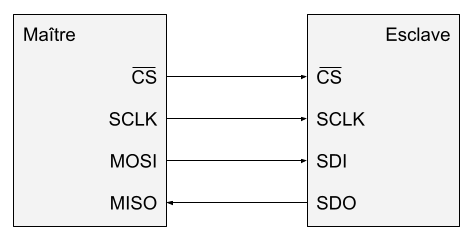
\includegraphics[scale=0.6]{./img/schema-spi.png}
    \caption{Liaison maître/esclave (SPI)}
    \label{fig:schemaspi}
  \end{center}
\end{figure}
%}}}

Maintenant que nous avons vu les principes du protocole, intéressons à la
simulation.

\subsubsection*{Émulation}

Pour réaliser la simulation de l'interface SPI, la démarche a était la même que
pour l'I²C. La mise en place d'une solution a été précédée d'une étude du
fonctionnement du code permettant d'utiliser le protocole.

La gestion du protocole dans le code est très similaire à celle de l'I²C. Il y a
un fichier dans le répertoire \verb|C32| contenant les fonctions basiques
du protocole. Là aussi, les lignes sont gérées à l'aide de variables globales
définies dans le fichier \verb|PicVariables|. Les fichiers plus haut niveau
du code commun ont permis de designer la machine a états au départ utilisée dans
la solution avec les threads puis réutilisée dans la nouvelle solution. Ici le
fonctionnement est un peu plus complexe qu'avec l'I²C. Pour faire une écriture
sur un composant, on commence par démarrer la communication puis on sélectionne
le composant auquel on souhaite s'adresser. Ensuite, on envoi un code qui va
permettre de choisir une action à réaliser. Parmi les actions possibles, il y a
la lecture, l'écriture ou encore la possibilité de supprimer des données
(erase). Il y a aussi un code permettant d'activer les droits d'écriture sur un
composant. Il faut donc activer l'écriture à chaque fois que l'on souhaite
modifier les données sur le stockage. Par exemple, pour faire une écriture sur
un composant, on commence par sélectionner la cible. Ensuite, on envoi le code
permettant d'activer l'écriture. Une fois fait, il faut redémarrer la
communication puis envoyer le code permettant d'écrire. Avant de pouvoir envoyer
les données à écrire, il faut déplacer le curseur du composant en envoyant une
adresse sur deux où trois octets, les données serons ensuite écrites à partir de
la nouvelle adresse du curseur. Lorsque l'on a fini d'envoyer les données, on
arrête la communication en repassant $\overline{CS}$ à 1.

Comme pour lI²C, il y a une fonction \verb|Control| qui est une machine à états
qui reprend les étapes décrites dans le paragraphe précédent. Là aussi, pour
utiliser la simulation, il faut modifier la fonction d'initialisation en
ajoutant les composant de façon similaire à l'I²C. À noter que la simulation de
la mémoire ne change pas et que l'on peut très bien configurer le même composant
à la fois sur lI²C et le SPI.
%}}}
\subsection{Système d'évènements}%{{{

À la fin de la conception de la simulation des interfaces I²C et SPI, il restait
un problème important. Ce problème était que l'on ne pouvait pas savoir depuis
les machines à états si les protocoles étaient utilisés correctement. Par
exemple, si un utilisateur oubliait de redémarrer la communication après le
déplacement du curseur pour une lecture I²C, il pouvait être très compliqué de
trouver l'origine du problème. Cela est du à la rigidité des machines à états
pour la simulation des interfaces de ces deux protocoles. Si les étapes ne sont
pas respectées à la lettre et que les bonnes fonctions ne sont pas appelées
dans le bon ordre le résultat est indéterminé. C'est un énorme problème étant
donnée le fait que l'on ne sait plus d'où viennent les erreurs, du code ou de la
simulation? C'est une question qu'il est légitime de se poser étant donné la
complexité de la simulation des interfaces du stockage.

Pour tenter de résoudre ce problème, un système d'évènement a été pensé. Ce
système est loin d'être parfait mais il peut éviter une partie des erreurs. Le
principe est que les machines à états de l'I²C et du SPI enregistrent des
évènements au fur et à mesure de l'exécution. Une fois que l'on a terminer une
action, on peut vérifier si les évènements enregistrés sont bon. Par exemple, on
peut essayer de faire un certain nombre de lectures avec le SPI. Le fichier du
SPI fournit une fonction qui permet de générer la liste des évènements attendus
pour $n$ lectures. Il suffit donc de comparer la suite d'évènements attendus à
celle des évènements enregistrés pour savoir s'il y a un problème. Cela
nécessite donc d'avoir un cas de test dédié qui fait la vérification des
évènements pour chacune des actions possibles.

TODO: détailler le système d'évènements
%}}}
\\
TODO: CONCLUSION sur le stockage
%}}}
\section{Protocoles monétiques}%{{{

Nous avons vu dans la partie précédente que les périphériques de stockage
étaient interfacés avec les protocoles I²C et SPI qui sont deux protocoles assez
courant dans les systèmes embarqués. La société CKsquare est spécialisée dans la
monétique et utilise donc beaucoup de périphériques interfacés avec des
protocoles spécifiques à ce domaine. Une grosse partie du stage a été passée à
la simulation d'interfaces utilisant deux protocoles très connus dans le milieux
de la monétique, le Cctalk et le MDB. Dans cette section, nous allons présenter
ces deux protocoles ainsi la solution proposée pour l'outil de test.

\subsection{L'interface Cctalk}%{{{
\label{interfacecctalk}

Une partie des composants utilisés sur la carte ont été interfacés avec le
protocole Cctalk. Dans cette section, nous commencerons par détailler les grands
principes de ce protocole puis nous verrons son implémentation par l'entreprise.
Enfin, nous expliquerons comment les périphériques Cctalk ont été simulés.

\subsubsection{Le protocole}

Le Cctalk est un protocole utilisé dans la monétique dont la première version a
été réalisée en 1996 par la société \verb|Coin Controls| basée en Angleterre
\cite{cctalkpt1}. Ce protocole est un \gls{protoserie} en \gls{halfduplex} créé
pour être utilisé pour des communications à débit moyen. En 2010 a été ajouté la
possibilité de chiffrer les trames (standard \gls{des}). Ce protocole est
destiné à être utilisé pour assurer la communication entre différents composants
reliés à une même carte.

Comme le SPI et l'I²C , le Cctalk fonctionne en mode maître et esclave. Ce
standard utilise un système de d'entête pour transmettre des commandes, par
exemple, l'entête 253 permet de demander son adresse à un composant. Il y a en
tout 256 entêtes différentes, numérotées de 0 à 255 ce qui permet la
transmission d'une entête sur un octet. Les entêtes de 20 à 100 sont réservées
pour les développeurs des applications utilisant le Cctalk, le reste est décrit
dans la documentation \cite{cctalkpt2}. Sur la figure \ref{tramecctalk} on peut
voir la composition d'une trame Cctalk qui comprend six éléments. Le premier est
l'adresse du composant ciblé par la trame (l'adresse du destinataire). Cette
adresse est suivit du nombre d'octets de données qui vont être envoyées. Ce
nombre étant transmis sur un octet, on ne pourra jamais transmettre plus de 255
octets de données. Ensuite, on envoi l'adresse de la source (le composant qui a
envoyé la trame) puis l'entête. Une fois l'entête envoyée, on transmet les
données puis le checksum qui va permettre de vérifier l'intégrité des données à
la réception.

% [trame cctalk] {{{
\begin{figure}[h!]
  \begin{center}
  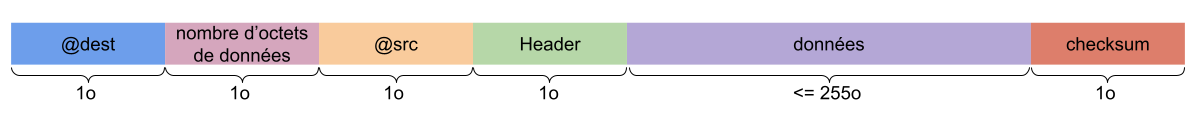
\includegraphics[scale=0.4]{./img/trame-cctalk.png}
  \caption{Trame Cctalk}
    \label{tramecctalk}
  \end{center}
\end{figure}
%}}}

Prenons l'exemple de l'écran créé par la société. Ici, on souhaite afficher du
texte sur l'écran, pour cela, on va utiliser l'entête 203 qui permet de
contrôler ce composant \cite{cctalkpt2}. Pour sélectionner l'action à réaliser,
il faut utiliser une sous-entête. Dans le cas de l'écran, il y a cinq
sous-entêtes permettant de réaliser des actions spécifiques à ce composant comme
effacer l'affichage par exemple. Dans notre exemple, on souhaite envoyer du
texte à afficher, pour ce faire, il faut utiliser la sous-entête 3. Ici, on va
donc envoyer une trame dont l'entête sera 203 et les données seront la
sous-entête 3 suivie du texte à afficher. L'écran doit normalement répondre par
un acquittement (entête 0).

Une exemple plus complexe est celui du système vocal. Ici, on va demander au
système vocal de lire un fichier audio. Là, il n'y a pas d'entête dédiée, la
société à donc utilisé une des entêtes mise à disposition des développeur:
l'entête 34. Cette entête ne sert que pour réaliser cette action, il n'y a donc
pas de sous-entête à envoyer. La trame qui sera transmise au système vocal sera
donc composée de l'entête 34 et des données requises à la lecture du fichier
comme le nom du fichier à lire, le nombre de répétitions, \dots Là aussi, le
composant doit répondre par acquittement.
\\~\\

Maintenant que nous avons expliqué le fonctionnement général du protocole, nous
allons nous intéresser au fonctionnement du code de l'entreprise.

\subsubsection{Le code de l'entreprise}

Dans le code de l'entreprise, le Cctalk est utilisé avec beaucoup de composants
comme un accepteur de billets, un lecteur de cartes, mais aussi le système vocal
de la borne ou encore l'écran tactile. Il y a un fichier pour chacun des
composants interfacé en Cctalk et ces fichiers permettent de gérer la partie
maître. Comme pour le stockage, la simulation a au départ été pensée pour se
situer au plus proche des fichiers du compilateur. Cela a nécessiter une
compréhension de toute la chaine d'instruction qui permet la transmission des
trames.

% note vérifier pour le role de master
Pour l'implémentation du Cctalk, il y a deux fichier principaux. Tout d'abord,
il y a le fichier \verb|CctalkMaster.c| qui permet de gérer la structure de
données qui modélise les commandes. Ce fichier possède aussi une fonction
\verb|Control| qui permet de gérer les \textit{Core Commands}, qui sont des
commandes généralement exécutées à l'initialisation et qui permettent d'obtenir
des informations sur les composant (constructeur, numéro de version, \dots).
Ensuite, il y a le fichier \verb|CctalkMasterSerial.c| qui gère la
communication. Ce second fichier sert de pont entre le code haut niveau des
communs et le code bas niveau des bibliothèques du \gls{pic}. Pour l'envoi des
trames, le fichier \verb|CctalkMasterSerial.c| utilise deux machines à états,
une \textit{haut niveau} et une autre \textit{bas niveau}. La machine à états
\textit{bas niveau} communique directement avec la bibliothèque de la carte,
elle se charge de la transmission et de la réception des données (envoi d'une
trame et réception de la réponse). La machine à états \textit{haut niveau} va
permettre l'envoi de différents types de trames. En effet, les trames Cctalk
transmises par la machine \textit{bas niveau} sont limités à 255 octets de
données. Pour palier à ce problème, la machine à états \textit{haut niveau}
permet d'envoyer des trames étendues. Le principe est de décomposer la trame à
envoyer en plusieurs sous trames. Pour que le composant sache que la trame est
une trame étendue, il faut envoyer deux trames supplémentaires avec une entête
de début et une entête de fin. L'envoi d'une commande se fait donc de la façon
suivante: on commence par appeler la fonction d'envoi de commande qui va ajouter
la nouvelle commande à une liste chaînée. Ensuite, le \verb|Control Manager| va
appeler la machine à états \textit{haut niveau} qui va utiliser l'autre machine
à état pour envoyer une ou plusieurs trames en fonction du type de trame à
transmettre (simple ou étendue).

L'implémentation par CKsquare du Cctalk propose beaucoup d'autres
fonctionnalités qui n'ont pas été traitées lors du stage. Par exemple, pour
limiter le \textit{polling} (interrogation d'un composant) sur certains
composants comme l'écran tactile, les développeurs ont mis en place un système
permettant à la carte de passer en mode esclave. L'interface du Cctalk est aussi
utilisée avec le TCPIP. En effet, le Cctalk est fait pour assurer la
communication entre les composants reliés à une même carte. Il peut arriver que
l'on ai besoin de lier des composants qui ne sont pas directement connectés et
pour ce faire on utilise le protocole TCPIP qui est le plus adapté. Le code de
la société propose une abstraction qui permet de gérer tous les composants en
utilisant seulement l'interface du Cctalk. Pour rendre cela possible, le code
utilise des drivers qui fonctionnent à l'aide de pointeurs de fonctions.

\subsubsection{Émulation des composants}

Comme expliqué dans la partie précédente, le répertoire \verb|Cctalk| contient
les fichiers qui permettent de gérer la partie maître pour chacun des
composants interfacés en Cctalk. Pour cette simulation, il fallait mettre en
place du code permettant de simuler le comportement des esclaves (donc des
composants) lors de la réception de trame. L'objectif des composants simulés est
simplement de répondre aux commandes Cctalk qu'ils reçoivent. Ces commandes
peuvent être automatiques ou paramétrées dans les tests. Un effet de bord
souhaitable pour la simulation est aussi la récupération de la trame reçue, de
sorte à ce que l'on puisse vérifier que les bonnes commandes sont envoyées dans
les tests.

Pour simuler les composants, il a été décidé d'utiliser un fichier par
composant. Lors du développement, il a été jugé plus simple et plus sage
d'adapter les principes utilisés lors de la simulation du stockage. Cette
décision a pour objectif d'apporter un maximum de cohérence dans le
fonctionnement de l'outil, cela pourra faciliter la maintenance ainsi que les
modifications. De plus, les tests réalisés sur le stockage ont prouvé le bon
fonctionnement de la solution. Enfin, pour faciliter la copie, les fichiers de
la simulation adoptent une forme standard que nous détaillerons plus loin. La
documentation met même à disposition un patron qu'il suffit de copier et de
modifier pour simuler un nouveau composant.

Comme pour le stockage, la simulation devait se situer au plus proche des
bibliothèques du compilateur. Cette approche a permis d'avoir une simulation
très réaliste qui pousse à l'utilisation du tous le code créé pour gérer le
Cctalk. C'est la première solution qui a été mise en place et qui a nécessité la
compréhension de toute l'implémentation du protocole. Bien qu'il soit
intéressant d'avoir une simulation réaliste permettant de faire des tests
d'intégration qui valident toute la chaine d'instruction, cette solution était
relativement complexe et poussait les tests à dépendre de l'entièreté du code.
Cela n'est pas souhaitable dans le cas où l'on veut faire des tests unitaires
sur un fichier sans se préoccuper du reste de l'implémentation. Cela est
intéressant car il permet de mieux repérer l'origine des problèmes car le code
testé est isolé, de ce fait, les échecs des tests sont dus uniquement aux
erreurs dans le fichier testé et non aux erreurs dans le reste du code. C'est
pour cette raison qu'une deuxième solution à été mise en place, permettant ainsi
de faire à la fois des tests unitaires et des tests d'intégrations. Pour mettre
en place cette solution, une version modifiée du fichier
\verb|CctalkMasterSerial.c| a été crée, dans cette version, les machines à états
sont supprimées. La sauvegarde de la trame reçue ainsi que l'envoi de la réponse
du composant est géré directement depuis la fonction qui permet d'envoyer les
commandes. De ce fait, quand un élément du code testé envoie une commande
Cctalk, cette dernière est enregistrée et la réponse est directement envoyée. On
ne passe donc plus par les machines à états, ni par les fichier du compilateur,
le code testé est donc bien isolé. Il est possible de passer d'une
implémentation de la simulation à une autre en définissant une constante
préprocesseur. À noter que c'est deux solutions ont été pensées pour être
interchangeables, de sorte à ce que les mêmes tests fonctionnent peu importe
l'implémentation de la simulation.

Comme nous l'avons mentionné dans un précédent paragraphe, tous les fichiers de
la simulation ont la même forme. Après plusieurs tests, une \textit{forme
standard} pour la simulation a été crée. Chaque fichier se compose des trois
fonctions suivantes:
\begin{itemize}
  \item[$\bullet$] \verb|Control|: Cette fonctions est utilisée avec la
    simulation bas niveau qui est la première solution crée. C'est une machine
    qui se compose de trois états. Dans le premier état, la machine fait la
    vérification de l'adresse sur la commande envoyée sur le bus par le code
    testé. Si cette adresse ne correspond pas à l'adresse du composant simulé,
    la machine s'arrête. Dans le cas contraire, la machine commence par
    récupérer la trame sur le bus pour que cette dernière soit accessible depuis
    les tests. Ensuite, elle envoi un écho qui permet de spécifier au maître que
    la trame a bien été reçu. Enfin, la machine à état envoi la réponse au
    maître en fonctions des données reçues, en utilisant les fonction du
    compilateur. % TODO: code en annexe
  \item[$\bullet$] \verb|Run|: Cette fonction permet de gérer la fonction
    décrite dans le point précédent. Elle fait une suite d'appels à la machine à
    états haut niveau de \verb|CctalkMasterSerial.c| pour déclencher l'envoi
    d'une commande avec les fonctions des bibliothèques du compilateur. Ensuite,
    elle fait appel à la fonction \verb|Control| qui récupère la commande du
    maître et envoie l'écho et la réponse. Enfin, elle fait une autre suite
    d'appels à la machine haut niveau pour enclencher la récupération de la
    réponse. La fonction \verb|Run| est à utiliser dans les tests à chaque fois
    qu'une commande doit être envoyée, elle permet gérer la simulation d'une
    communication entre la carte et un composant. À noter que cette fonction
    n'est utile qu'avec la version bas niveau (version où l'on test tout le
    code), cependant, il existe une version vide de cette fonction qui permet de
    ne pas avoir à modifier les tests quand on passe de la version bas niveau à
    la version haut niveau.
  \item[$\bullet$] \verb|HandleResponse|: Cette dernière fonction est utilisée
    avec la version haut niveau. Comme expliqué précédemment, dans cette
    version, tout est géré depuis la fonction \verb|CmdSnd| de la version
    modifiée pour les tests du fichier \verb|CctalkMasterSerial.c|. Ici, il n'y
    a qu'un seul fichier pour tout les composants ce qui pose problème pour les
    réponses prés définies. Pour pouvoir paramétrer des réponses pour plusieurs
    composants, on passe par un pointeur de fonction qui pointe sur la fonction
    \verb|HandleResponse| du composant testé. Cette fonction se compose juste
    d'un \verb|switch| qui va envoyer une réponse en fonction des données
    reçues. À l'initialisation de chaque test, il faut affecter l'adresse d'une
    fonction \verb|HandleResponse| à la variable globale \verb|HANDLE_RESPONSE|.
\end{itemize}

TODO: code en annexe

\subsubsection{Exemple de test}

TODO: conclusion sur le cctalk

%}}}
\subsection{L'interface MDB}%{{{

Dans la partie précédente nous avons traité le fonctionnement du protocole
Cctalk et nous avons aussi vu comment les composants Cctalk ont été simuler pour
faire fonctionner les tests. Dans cette partie, nous allons traiter un autre
protocole utilisé avec d'autre composants, le protocole MDB. À noter que le
fonctionnement du MDB dans le code de CKsquare ainsi que celui des composants
simulés est très similaire au Cctalk, il y aura donc beaucoup de parallèles fait
avec la partie précédente.

\subsubsection{Le protocole}

Le protocole MDB a été créé dans les années 1980 par la société \textit{CoinCo}
et a au départ été très utilisé dans les distributeurs automatiques de
\textit{Coca-Cola} \cite{enwiki:1094073752}. Le protocole est devenu
\textit{open-source} en 1992 et la \textit{National Automatic Merchandising
Association} (NAMA) a réalisé la première version du standard en 1995.

Comme le Cctalk, le protocole MDB fonctionne en mode maître et esclave où la
carte électronique est le maître qui contrôle les périphériques qui eux sont les
esclaves. Pour que le maître puisse transmettre des ordres aux esclaves, le MDB
utilise un système de commandes et de sous-commandes.

Comme le précise la documentation du protocole \cite{mdbdoc}, la transmission
des informations avec le MDB se fait sur neuf bits. Parmi ces neuf bits, il y a
huit bits qui permettent de transmettre des données et le dernier bit et un bit
de mode. Lorsque le bit de mode est à 0, les huit premiers bits contiennent des
données. S'il est à 1, alors les huit premiers bits peuvent contenir l'adresse
d'un composant cible (l'adresse du composant auquel s'adresse le maître), une
commande spéciale ou un checksum. Les commandes spéciales sont ACK
(acquittement), NAK (non acquittement) et RET (demande de répétition). Un octet
d'adresse contient généralement aussi une commande: un \textbf{ou} logique est
fait entre l'adresse du composant et la commande à envoyer. À noter que le
standard impose des adresses spécifiques pour chaque type de périphérique. Par
exemple, un accepteur de billet doit avoir pour adresse \verb|0x30|. Les
commandes envoyées avec l'adresse permettent de donner des ordres aux
périphériques et chaque type de périphérique possède son propre jeux de
commandes. Les commandes correspondent à des catégories assez génériques, par
exemple pour l'accepteur de billet, \verb|0x03| permet d'interroger le composant
(pour savoir s'il y a un billet a été accepté par exemple). Ensuite, pour
spécifier une action à réaliser on envoi à nouveau neuf bits avec le bit de mode
à 0 et une sous-commande dans les données. On peut envoyer plus de données si
besoin mais les sous-commandes doivent toujours apparaitre au début.

Traitons l'exemple du début de la validation d'une vente simple avec un
périphérique de paiement sans contactes. Ce scénario est décrit dans la
documentation \cite[p.~169]{mdbdoc}. Ici, la carte va commencer par interroger
le composant en utilisant la commande \textit{poll} (code \verb|0x02|). Les
systèmes de paiement sans contactes ont pour adresse \verb|0x10| ou \verb|0x60|,
ici, la première trame sera donc composée de neuf bits. Le bit de mode sera à 1
car on souhaite interroger un composant, et pour ce faire il faut envoyer son
adresse sur le bus. La valeur des huit bits suivant est le résultat d'un ou
logique entre la commande \verb|0x02| et l'adresse du composant donc \verb|0x12|
ou \verb|0x62|. Ensuite, le composant va renvoyer neuf bits où le bit de mode
sera à 0 et la huit bits suivant contiendront la commande \verb|0x03|, ce qui
permet de démarrer une session (échange de trames). Une fois la session
démarrée, la carte va demander s'il y a une ventre à traiter, pour ce faire, on
utilise la commande \textit{Vend} (\verb|0x03|) et cette dernière s'accompagne
d'une sous-commande \textit{Vend Request} (\verb|0x00|). On peut noter ici que
pour un même code, la commande correspondante sera différente en fonction de
l'émetteur de la trame (maître ou esclave). La nouvelle trame sera donc composée
de 18 bits: \verb|0x113| (bit de mode à 1, adresse du composant \verb|0x10| et
commande \verb|0x03|) \verb|0x000| (bit de mode à 0 et sous-commande
\verb|0x00|). Ensuite le périphérique doit répondre par la commande
\textit{ACK}, donc ici, le bit de mode est à 1 et les huit bits suivants sont
nuls. Comme mentionné plus haut, le reste du scénario est décrit dans la
documentation du MDB.

Maintenant que nous avons décrit les bases du protocole, intéressons nous au
code de l'entreprise. On pourra ensuite étudier le fonctionnement de la
simulation des composants.

\subsubsection{Le code de l'entreprise}

L'implémentation du MDB suis le même principe que celle du Cctalk sauf qu'ici,
il n'y a pas plusieurs types de trames à gérer, le code est donc plus simple. Le
protocole est géré par le fichier \verb|MDBApi.c| qui contient la fonction
\verb|CmdSnd| qui permet d'enregistrer les commandes à envoyer. Ce fichier
contient aussi une fonction \verb|Control| qui correspond à la machine à état
principale. Comme pour le Cctalk, la fonction \verb|Control| interagir avec les
fonctions du fichier \verb|serial.c| qui fait partie des bibliothèques du
compilateur. La fonction commence dans un premier temps par envoyer les
différentes parties de la trame (adresse, données puis checksum), puis attend
que la réponse soit disponible.

Lorsque l'on souhaite envoyer une trame, on utilise la fonction \verb|CmdSnd|,
qui va marquer la commande qu'elle reçoit en paramètre comme étant prête à être
envoyée. Il n'y a pas de liste chaînées ici, toutes les commandes sont stockées
dans un tableau et elles sont affectée aux différents composants lorsqu'ils sont
enregistré (a l'initialisation du programme). Toutes les commandes sont
accessibles depuis le fichier \verb|MDBApi.c| et elles sont simplement marquées
pour être envoyées. Lorsque le \verb|ControManager| appelle la fonction
\verb|Control| du fichier, cette dernière transmet toutes les commandes marquées
et récupère toutes les commandes.

\subsubsection{Émulation des composants}

La simulation des composants interfacés en MDB a été réalisée dans la continuité
de ce qui a été fait pour le Cctalk. Là aussi, on a un fichier par composant, et
les fichiers ont une forme similaire.

Comme le Cctalk, la simulation MDB est disponible en deux versions, une
\textit{haut niveau} qui utilise une version modifiée du fichier \verb|MDBApi.c|
et une version \textit{bas niveau} qui passe par toute la chaine d'instructions
jusqu'aux bibliothèques du compilateur. La grosse différence avec le Cctalk en
terme d'utilisation est que la simulation ne propose pas de réponses
prés-définies aux commandes envoyées par la carte. En effet, comme il peut y
avoir beaucoup de réponses différentes pour une même commande, il a été décidé
que les réponses des composants devaient être configurées à chaque fois. Cela
signifie que dans les tests, il faut configurer une réponse avant l'envoi d'une
commande. On a donc une grande maitrise depuis les tests du fait qu'il est très
simple de tester toutes les possibilités dans plusieurs tests. La forme des
fichiers des composants simulés est aussi similaire à celle des fichiers du
Cctalk. Il y a une fonction \verb|Control| qui est utilisée avec la version
\textit{bas niveau} et qui a la même utilité que la fonction du Cctalk. Là
aussi, il y a une fonction \verb|Run| qui comme pour le Cctalk permet de lancer
la simulation du composant depuis les tests lorsque la version \textit{bas
niveau} est utilisée. Comme il n'y a pas de réponse prés-définies, il n'y a pas
de fonction \verb|HandleResponse|. L'obligation de configurer toutes les
réponses aux commandes rend certains tests complexe à écrire, c'est pour cela
qu'un système de scénarios a été ajouté au MDB, ce système est décrit dans la
section \ref{sysscenar}.

TODO: code en annexe

\subsubsection{Système de scénarios}
\label{sysscenar}

Comme dit précédemment, les réponses aux commandes étant trop complexes, la
simulation des composants MDB ne propose pas de moyen d'avoir des réponses prés
définies comme avec le Cctalk. Par contre, ici, la documentation fournit des
scénarios qui décrivent des échanges de trames entre le maître et les
composants. Pour pouvoir vérifier si ces échanges de trames sont possibles avec
le code de l'entreprise, un système de scénarios a été mis en place. Ce système
permet de définir une suite d'envoi de commande par le maître et de réponse par
l'esclave. À chaque fois que le composant simulé reçoit une trame, il vérifie
que cette dernière correspond à celle prévue par le scénarios avant de
transmettre la réponse. Si la trame reçue par l'esclave ne correspond pas à ce
qui été prévue par le scénario, on fait échouer le test avec un \verb|exit(1)|.
À noter que seul le test sur le scénario joué échoue et les tests suivants sont
exécutés correctement car avec notre framework, chaque test s'exécute dans son
propre thread. Cela simplifie grandement l'écriture des tests puisqu'il n'y a
pas besoin de paramétrer les réponses du composant ni même de faire des
assertions puisque si le test passe c'est que le scénarios a été joué
correctement, sinon, c'est qu'il a planté. Ce système de scénario est donc un
moyen très simple de valider le code CKsquare pour un type de périphérique.

L'implémentation de ce système est très simple, les scénarios sont composés
d'étapes et chaque étape est modélisée par une structure. Les étapes sont
stockées dans un tableau global. Lorsque l'on souhaite jouer un scénario, on
appel la fonction \textit{play} correspondante au début du test. Cette dernière
fait un enregistrement d'étapes dans le tableau global. Ensuite, l'envoi
réponses et la vérification des commande envoyées par la carte est automatique,
il suffit juste d'appeler les fonctions du code pour passer par toutes les
étapes du scénario. À noter que la plupart du temps, il faut initialiser les
machines à états au préalable car les étapes de démarrage ne sont pas prises en
comptes dans les scénarios.

TODO: exemple de scénario et de test\\
TODO: code en annexe

\subsubsection{Exemple de test}
%}}}
%}}}
\section{Les historiques}%{{{

Dans cette section, nous allons nous intéresser à la gestion des historiques
(historique de paiement, \dots). Ils sont stokés en mémoire sur la carte dans
une base de données circulaire et ils sont régulièrement sauvegardé sur un
serveur. C'est un élément important car la sauvegarde des historiques est
juridiquement obligatoire quand ils concernent la monétique (loi finance de
2016). Dans cette partie, nous commencerons, dans un premier temps, par
détailler le fonctionnement de la structure de données et des tests qui ont
été fait dessus. Dans un second temps, nous traiterons l'envoi des
historiques sur le serveur de CKsquare.

\subsection{Les CDBs}

Tous les historiques sont stockés dans un base de donnée circulaire (CDB
signifie \textit{Circular Data Base}). La première partie des tests concernant
les historiques va porter sur la validation du bon fonctionnement de cette base.
Un point important concernant cette structure est que les CDB sont stockées en
mémoire (généralement sur des eeproms). Les tests qui vont être réalisés sur
cette structure vont permettre de pleinement utiliser l'émulation du stockage.
Ils vont donc constituer un exemple intéressant qui pourra être décrit dans la
documentation.\\

Comme mentionné dans le paragraphe précédent, un CDB est une une base de donnée
circulaire. Un CDB est une structure qui se compose d'un tableau, d'un compteur
d'éléments, d'une tête et d'une queue. La tête correspond à la première donnée
insérée et la queue à la dernière. Les CDB sont sauvegardés en mémoire sur des
eeproms ou des flashs en fonction de la configuration. Il y a une seule
interface (fichier d'entête) pour deux implémentation différentes utilisant les
deux types de périphériques de stockage et on peut passer d'une implémentation à
une autre avec la configuration. Il est important de pouvoir tester les deux
implémentations, par contre, étant donné que les fonctions ont le même nom, on
ne peut pas compiler tous les fichiers en même temps (une interface et deux
implémentations). C'est pour cette raison que l'on génère deux exécutables
différents, où chaque exécutable est compilé avec une configuration différente.
Comme expliqué dans la section \ref{cmake}, pour passer d'une configuration à
une autre, on utilise des constantes préprocesseurs définies à la compilation.
Il y aura donc aussi deux tests différents, un pour les flash et un pour les
eeproms.

Traitons à présent un exemple de test sur un CDB dont le code est visible sur le
listing \ref{extestinsertcdb}. Ici, on test l'insertion d'éléments dans une
flash. Pour réaliser ce test, on utilise plusieurs fonctions annexes. La
fonction \verb|TESTCDB_IndexToAddrRelative| prend en paramètre un CDB, un indice
et une référence sur une adresse. Elle permet de récupérer l'adresse de
l'élément du CDB à l'indice donnée dans la flash. Pour ce test, on utilise des
historiques de paiement et on utilise la fonction
\verb|TESTCDB_RandomBufferGenerate| pour générer un élément aléatoire à insérer
dans le CDB. Dans un premier temps, on insère un élément dans la base et on
regarde si les données ont bien été écrites dans la flash. Ensuite, on vérifie
que les données du CDB sont aussi écrites au début de la mémoire. En effet,
lorsque l'on redémarre la carte, on a besoin de récupérer l'état de la base de
données (le nombre d'élément stockés, \dots). Pour pouvoir faire cela, la
structure qui permet de gérer le CDB est écrite en début de mémoire
(\verb|CDB->Control|). Une fois que l'on vérifié qu'une insertion dans le CDB
fonctionnait, on teste s'il est possible de remplir la base en ajoutant le
maximum d'éléments à l'aide d'une boucle. À noter qu'à chaque fois, on vérifie
que l'élément (toujours généré aléatoirement) est bien écrit dans la mémoire. À
la fin, on test que le CDB est bien plein.

\begin{listing}[ht!]
\begin{minted}{C}
Test(CDB_Test, TESTCDB_Add, .init = TESTCDB_Setup, .fini = TESTCDB_Teardown)
{
    uchar Buff[sizeof(TITEM_PAYMENT)];
    ulong BeginingAddr = ((TCDBONFLASH_CONTROL * )CDB->StorageData)->NextAddr + 1;
    TFLASH_ADDR Addr;
    int Cpts;

    TESTCDB_IndexToAddrRelative(CDB,0,&Addr);
    TESTCDB_RandomBufferGenerate(Buff,sizeof(TITEM_PAYMENT));
    cr_assert(true == CDB_Add(CDB ,Buff));
    // le cdb a bien été écrit dans la flash
    cr_assert(eq(u8[sizeof(TITEM_PAYMENT)],TESTMEM_FLASHM[0] + Addr,Buff));
    // on vérifie que le control est bien écrit au début
    CDB->Control.CounterChange--;
    cr_assert(eq(u8[sizeof(CDB->Control)],
                 TESTMEM_FLASHM[0] + BeginingAddr,
                 (uchar*) &CDB->Control));
    CDB->Control.CounterChange++;

    /* remplissage de la base */
    for (Cpts = 1; Cpts < CDB->RecordMax; ++Cpts) {
        TESTCDB_RandomBufferGenerate(Buff,sizeof(TITEM_PAYMENT));
        cr_assert(true == CDB_Add(CDB ,Buff));
        TESTCDB_IndexToAddrRelative(CDB,Cpts,&Addr);
        cr_assert(eq(u8[sizeof(TITEM_PAYMENT)],TESTMEM_FLASHM[0] + Addr,Buff));
    }
    cr_assert(true == CDB_IsFull(CDB));
}
\end{minted}
\caption{Test d'insertion dans un CDB}
\label{extestinsertcdb}
\end{listing}

Ce test permet de valider l'insertion d'éléments dans un CDB et il y a d'autres
tests qui permettent de valider d'autres fonctionnalités ces bases de données
comme la suppression par exemple. Ici, on peut voir que la simulation des
périphériques de stockage fonctionne bien et que cette dernière est assez simple
à utiliser dans les tests. On voit bien que l'on peut aisément vérifier si la
mémoire a été modifiée en utilisant les outils du framework. Ce sont des
résultats positifs qui montrent la viabilité de l'outil de test.\\

Maintenant que nous avons abordé le fonctionnement des CDBs ainsi que les tests
qui sont associés à cette structure de données, nous allons nous intéresser au
test de la sauvegarde des historiques sur le serveur.

\subsection{Sauvegarde des historiques}

Dans la section précédente, nous avons traité l'utilité et le fonctionnement des
CDB, étudions le problème de l'envoi des historiques sur le serveur. À noter que
c'est un problème  concernant l'envoi des historiques de paiement sur le
\textit{CKWash} (serveur de CKsquare) qui a donné aux développeurs l'idée de ce
stage.\\

Pour envoyer les historiques sur le serveur, le \verb|ControlManager| va
régulièrement faire appel à une fonction \verb|Control| qui va envoyer tous les
nouveau historiques sur le \textit{CKWash} et les supprimer des CDB. Cette
fonction se trouve dans le fichier \verb|CksproHisSend.c| Pour transmettre les
historiques, on utilise un protocole créé par la société qui est le protocole
\textbf{CKspro}. Ici, seule une version haut niveau de la simulation à été mise
en place car le code qui permet de gérer la transmission des données utilise
directement des éléments bas niveau comme le TCPIP. Ces éléments étant
relativement complexes et assez peu utilisés dans le code, ils n'ont pas été
traités durant le stage car cela aurait pris trop de temps.

Pour pouvoir tester l'envoi des commandes, une version modifiée du fichier
chargé de la gestion du protocole CKspro a été créée. Comme pour le Cctalk et le
Mdb, la fonction \verb|Control| du fichier n'est pas utilisée et la fonction
\verb|CmdSnd| a été modifiée. Cette dernière récupère les commandes envoyées et
les sauvegarde dans une variable globale accessible depuis les tests. Pour
tester si les commandes sont bien envoyées, on place des éléments dans un CDB et
on appelle la fonction \verb|Control| du fichier \verb|CksproHisSend.c| qui va
envoyer tous les éléments enregistrés dans la base. On peut ensuite tester si
les commandes envoyées correspondent aux données qui avaient été enregistrées en
vérifiant que les identifiants stockés dans les trames sont les mêmes que ceux
des éléments dans CDB. À noter qu'ici, un test assez réaliste a été écrit pour
vérifier que l'outil permet bien de créer un test capable de détecter le
problème qui a pousser la société à créer ce sujet de stage. Le problème été
survenu plusieurs fois à cause de mauvaises manipulations de git, ce qui aurait
pu être détecté facilement avec une pipeline. Il venait d'une erreur de
configuration qui faisait que dans la fonction \verb|Control| de l'envoi des
historiques, une fonction était appelée à la place d'une autre. Ce problème
était assez difficile à détecter avec de simples tests puisqu'il apparaissait
uniquement lorsque le CDB était remplit plusieurs fois (problème d'index dans le
CDB). Pour détecter ce problème, on remplit le CDB, on envoie tous les
historiques et on refait ces opérations en vérifiant à chaque fois que tous les
éléments sont envoyés. Le test fonctionne bien et sont code est disponible à
l'annexe \ref{}.

Les tests sur l'envoi des historiques sont relativement complexes dans le sens
où ils doivent utiliser plusieurs des éléments mis en place par l'outil de test.
En effet, ici, le test doit utiliser la version modifiée du fichier
\verb|CKspro.c| et les modifications apportées à ce fichier suivent les mêmes
principes que pour le Cctalk et le MDB. En plus de la modification de fichier
pour isoler les éléments du code testé, les tests sur l'envoi d'historiques
utilisent les CDB et donc la simulation du stockage. Le fait d'avoir un résultat
positif sur un test qui utilise une grande partie du code et autant des éléments
mis en place par l'outil est très positif. Cela permet donc de valider en grande
partie les techniques et méthodes employées durant le stage. Enfin, un autre
point intéressant concerne la difficulté d'écriture des tests. En effet, les
tests ne sont pas triviaux à écrire, cependant, leur complexité vient plus de
celle du code testé que de l'outil.
%}}}
\section{Mise en place de la pipeline}

Dans cette section nous allons voir comment a été mise en place la pipeline
Gitlab.

La configuration de la pipeline contient deux \textit{jobs}, un \textit{job} de
compilation et un \textit{job} de test. Il y a une contrainte de précédence
entre la compilation et les tests.

Pour la compilation, on commence par installer le nécessaire pour compiler avec
le gestionnaire de paquets de la pipeline (\textit{Aptitude}). Cela comprend les
outils comme \verb|gcc| et \verb|cmake| mais aussi le framework de test. Ici, on
utilise l'image docker par défaut de Gitlab (\verb|ruby:3.1|) car il n'y a pas
beaucoup de paquets à installer mais il serait possible d'utiliser une image
plus complète ou d'en créer une. Le projet \verb|dev_pic| est dépendant du
projet \verb|commun_global| qui comme expliqué en début de rapport correspond au
code partagé entre tous les projets. Pour accéder à ce projet depuis la
pipeline, il y a deux solution, la première consiste à utiliser un \gls{smodg}.
Le défaut de cette méthode est qu'elle nécessite la gestion d'un sous module
dans les communs. De plus, cette solution n'est pas très logique et
complexifierait énormément la gestion du projet car \verb|dev_pic| est déjà un
sous module des projet de l'entreprise. La seconde méthode est beaucoup plus
simple puisqu'elle consiste juste en le clonage du projet \verb|commun_global|
dans la pipeline. Pour pouvoir cloner un projet privé, on utilise un \textit{job
token} accessible depuis la configuration à l'aide d'une variable. Une fois que
l'on a téléchargé toutes les dépendances du projet, on met en place CMake et on
compile les tests.

TODO: reste des explications\\
TODO: mettre la config\\

Dans le second \textit{job}, on va lancer les tests. On commence par réinstaller
toutes les dépendances.

La création de cette pipeline a clos la première partie du stage qui concernait
la création d'un outil de test sur la branche principale du code C. Le travail
suivant a consisté en l'adaptation de l'outil sur la branche évènementiel qui
est l'autre branche du projet \verb|dev_pic| que nous avons détaillé dans la
section \ref{brancheevent}. Dans la partie suivante nous allons nous intéresser
aux modifications apportées à l'outil pour que ce dernier fonctionne sur la
seconde branche.

\section{Les tests sur la branche de l'événementiel}

\section{Le projet de test sur la partie Qt}

\subsection{Nouveau framework}

- Premier framework compatible cpp pour rien
- collaboration avec samuel qui trouvé un framework plus adapté à Qt

\subsection{Les problèmes du code Qt}

- fonctions control privées et actionnées avec des évènements timer
- solution avec des wait pas idéale
- mocking pas toujours possible ou trop complexe
- pas de solution pour controler les timers
- solution du define pas utilisée mais envisagée
- fonctionnement du Méta Object Compiler pas évident au départ

\subsection{La simulation}

- code objet plus simple.

\section{Déroulement du projet}

Dans cette dernière section, nous allons nous intéresser aux méthodes de
trivial et aux outils utilisés durant ce stage. Nous ferrons ensuite la
comparaison entre le planning prévisionnel et le planning réel.

\subsection{Les outils utilisés}%{{{

Dans cette partie, nous allons faire une revue des outils utilisés pendant le
stage. Les outils les plus utilisés ne seront pas détaillé, par contre, cette
partie a pour but de mettre en lumière les avantages qu'il y a à connaitre et
configurer ses outils de travail.

\subsubsection{Gestion de version}

Pour la réalisation du projet, le gestionnaire de version utilisé été Git. À
noter que la société n'utilise Git que depuis un ans, le gestionnaire de version
qu'ils utilisaient avant été SVN.

L'avantage de Git est qu'il est assez simple d'utilisation mais propose tout de
même des fonctionnalités très complexes. De plus, par rapport à SVN, Git est
décentralisé et permet de faire des branches ce qui a été très utile pour éviter
que le projet de tests pose problème.

La philosophie de travail utilisé a consisté en une version réadapté de Gitflow.
Le principe de Gitflow est d'avoir une branche \verb|master| qui va
contenir les versions du projet. Ensuite, il y a une branche \verb|dev| qui
est utilisée pendant le développement. La branche \verb|dev| contient du
code fonctionnel mais qui n'est pas encore déployé sur \verb|master|. Entre
les branches \verb|master| et \verb|dev| il doit normalement y avoir
une branche \verb|release| qui contient des prés-versions mais elle n'a pas
été utile ici. Enfin, à partir de la branche \verb|dev|, on créer des
branches de \verb|features| sur lesquelles on développe les nouvelles
fonctionnalités. Étant donné que le travail se faisait seul, le fait d'utiliser
Gitflow avec autant de branche n'était pas vraiment nécessaire. Cependant, cette
méthode permet d'être très organisé. Cela permet par exemple de toujours avoir
du code fonctionnel présentable à un collègue. De plus, cette organisation des
branches permet de ne pas se perdre et de ne jamais caser du code fonctionnel.
L'avantage des branches est que l'on peut facilement faire des tests pour savoir
si une solution est réalisable.

À noter que l'équipe de développement de CKsquare utilise l'application
\textbf{gitahead}. Cette application n'a pas été utilisée pendant le
développement du projet de tests. C'est l'interface en ligne de commande de Git
qui a été privilégiée ainsi que l'utilisation du plugin \textbf{fugitive} sur
neovim.

\subsubsection{GDB}

TODO: Un des objectifs de ce stage été de progresser sur l'outil GDB.\\
TODO: utilisation avancée de gdb\\
TODO: configuration de gdb

\subsubsection{IDE}

TODO: nvim -> vim-fugitive, clangd, l'intégration de gdb ... Présentation rapide
de ma configuration.
%}}}
\subsection{Rédaction de la documentation}%{{{
\clearpage
%}}}
\subsection{Planification des tâches}%{{{

Les tâches prévues lors du stage étaient les suivantes. Au départ, il était
prévu de faire le choix du framework de tests puis de faire une revue des
éléments du code à tester. Ensuite, il était prévu de faire des tests sur des
fichiers simples pour s'habituer au code de l'entreprise et aussi permettre de
compiler une première partie du projet. Une fois le projet pris en mains,
l'objectif était de s'attaquer aux grandes parties qui étaient tout d'abord le
stockage, puis le Cctalk et le MDB. Les historiques devaient être testés à la
fin du fait de leur dépendance au stockage. Il était aussi prévu de réaliser de
la documentation en parallèle tout au long du projet.

% [expected gantt] {{{
\begin{figure}[h!]
  \begin{center}
  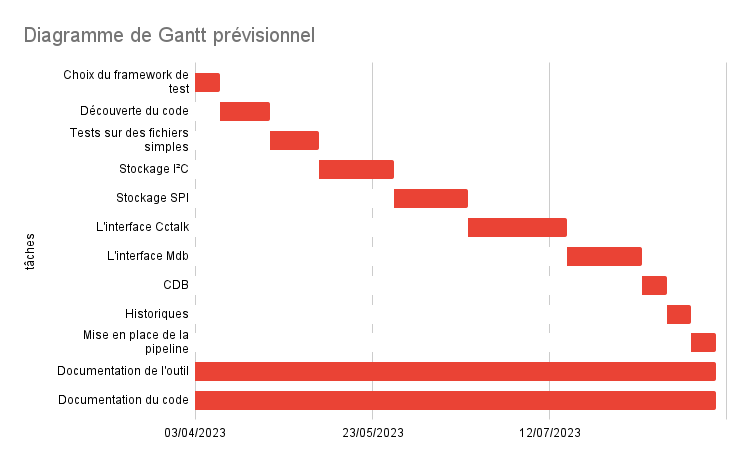
\includegraphics[scale=0.6]{./img/expected-gantt.png}
  \caption{Diagramme de Gantt prévisionnel}
  \end{center}
\end{figure}
%}}}

L'organisation de ces tâche a été faite sans connaissance de la complexité du
code. Certains des composants de l'outil final ont été refait plusieurs fois car
les résultats ne satisfaisaient pas les critère nécessaire à leur validation.
C'est le cas du stockage où au départ il avait été fait le choix d'utiliser des
threads, un choix qui a été remis en cause par la suite. Un autre exemple serait
celui du Cctalk dont certaines parties ont été réécrites suite à
l'implémentation de l'émulation des composants MDB pour ajouter plus de
cohérence. Malgré le fait que certains éléments ont été refaits, le
développement a pris moins de temps que prévu. Les tâches ont été surévaluées du
fait du manque de connaissances sur certains éléments comme les protocoles par
exemples.

NOTE: diagramme actuel

% [current gantt] {{{
\begin{figure}[h!]
  \begin{center}
  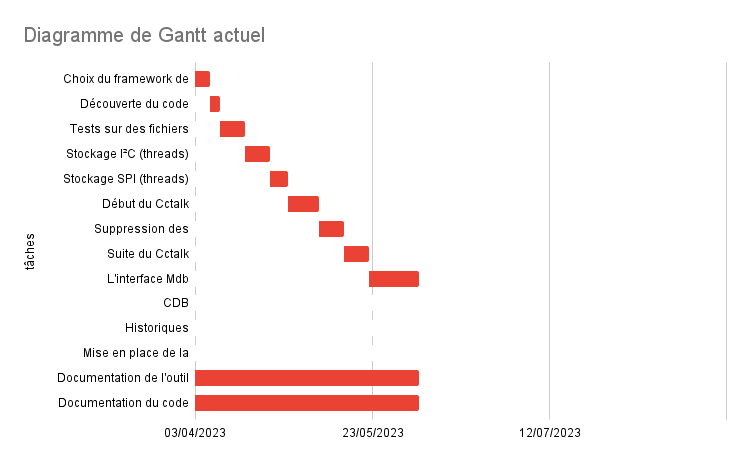
\includegraphics[scale=0.6]{./img/current-gantt.png}
  \caption{Diagramme de Gantt actuel.}
  \end{center}
\end{figure}~\\
%}}}
%}}}
\clearpage
%***************************************************************************}}}
% Résultats et discussions *************************************************{{{
\part{Résultats et discussions}

\section{L'outil final}

Description de l'outil final réalisé à la fin du stage.

TODO: Rétrospective sur le choix du framework (problème macros, ...).

\clearpage

\section{Discussion et perspectives}

Regard sur ce qui a été fait et comment cela a été fait (parler de l'échec
des threads, manque de bibliographie, ...). Parler de ce qui reste à faire ou a
améliorer.

\clearpage

\section{Développement durable}

NOTE: Je ne sais pas comment nommer cette partie, elle doit correspondre à la
réflexion sur les enjeux actuels liés à la responsabilité sociétale et
environnementale demandée par la CTI.

\clearpage

\section*{Conclusion}
\addcontentsline{toc}{section}{Conclusion}

CONCLUSION

%***************************************************************************}}}

%------------------------------------------------------------------------------%
%                                 bibliographie                                %
%------------------------------------------------------------------------------%

\section{Résumé biblio (WARN: section temporaire)}

Test affichage biblio:

\begin{itemize}
  \item \cite{enwikiframeworks}: liste des frameworks sur Wikipédia
  \item \cite{enwikifixtures}: définition fixture Wikipédia
  \item \cite{teststatemachines}: tester des machines à états
  \item \cite{mankar2014review}: présentation du protocole I²C
  \item \cite{dhaker2018introduction} et \cite{li2014design}: présentation du
    protocole SPI
  \item \cite{articleembeddedtests}: test de systèmes embarqués en utilisant de
    la simulation. Très différent du projet mais il y a des point intéressants.
  \item \cite{engblom2015continuous}: simulation pour CI sur systèmes embarqués
  \item \cite{maartensson2016continuous}: intégration continue sur les systèmes
    embarqués.
  \item \cite{hamill2004unit}: livre sur les frameworks de tests (p 42: mocking)
  \item \cite{cctalkpt1}, \cite{cctalkpt2},\cite{cctalkpt3}: trois premières
    parties de la doc cctalk
  \item \cite{mdbdoc}: doc mdb
\end{itemize}

\clearpage{}
\pagestyle{empty}
\printbibliography[keyword={paper},title={Bibliographie}]
\printbibliography[keyword={web},title={Webographie}]

%------------------------------------------------------------------------------%
%                                  glossaire                                   %
%------------------------------------------------------------------------------%
\clearpage
\printglossaries

%------------------------------------------------------------------------------%
%                                   annexes                                    %
%------------------------------------------------------------------------------%
\appendixwithtoc

% Extraits de codes pour les frameworks -------------------------------------{{{
\clearpage{}
\section{Extraits de codes pour les frameworks}\label{appendix:frameworks-code}

\subsection*{Check}

\begin{listing}[ht!]
\begin{minted}{C}
#include <check.h>

START_TEST(test_name)
{
  ck_assert(1 == 1);
  ck_assert_msg(2 == 2, "Should be a success");
}
END_TEST

Suite *simple_suite(void) {
  Suite *s;
  TCase *tc_core;
  s = suite_create("suite name");
  tc = tcase_create("test case name");
  tcase_add_test(tc_core, test_name); // adding tests
  suite_add_tcase(s, tc_core); // create the suite

  return s;
}

int main(void) {
  int number_failed;
  Suite *s;
  SRunner *sr;
  s = simple_suite();
  sr = srunner_create(s);
  srunner_run_all(sr, CK_NORMAL);
  number_failed = srunner_ntests_failed(sr);
  srunner_free(sr);
  return (number_failed == 0) ? 0 : 1;
}
\end{minted}
\caption{Check: Exemple simple}
\label{check-example}
\end{listing}

\clearpage{}
\subsection*{CUnit}

\begin{listing}[ht!]
\begin{minted}{C}
/******************************************************************************/
/*                                   tests                                    */
/******************************************************************************/

void test_function(void) {
  CU_ASSERT(0 == 0);
}

/******************************************************************************/
/*                              setup & teardown                              */
/******************************************************************************/

int init_suite(void) {
  return 0; // -1 for error
}

int clean_suite(void) {
  return 0; // -1 for error
}

/******************************************************************************/
/*                            lancement des tests                             */
/******************************************************************************/

int main(void)
{
  CU_pSuite pSuite = NULL;
  /* initialize the CUnit test registry */
  if (CUE_SUCCESS != CU_initialize_registry())
    return CU_get_error();
  /* add a suite to the registry */
  pSuite = CU_add_suite("suite name", init_suite, clean_suite);
  if (NULL == pSuite) {
    CU_cleanup_registry();
    return CU_get_error();
  }
  /* Adding to the test suite */
  if ((NULL == CU_add_test(pSuite, "description", test_function)))
  {
    CU_cleanup_registry();
    return CU_get_error();
  }
  /* Run all tests using the CUnit Basic interface */
  CU_basic_set_mode(CU_BRM_VERBOSE);
  /* Run tests */
  CU_basic_run_tests();
  /* withdraw error number (for returning to pipeline) */
  unsigned int nb_errors = CU_get_number_of_suites_failed();
  /* registry cleanup */
  CU_cleanup_registry();
  return 0;
}
\end{minted}
\caption{CUnit: exemple simple}
\label{cunit-example}
\end{listing}

\clearpage{}
\subsection*{Criterion}

\begin{listing}[ht!]
\begin{minted}{C}
// test basique
Test(suite_name, test_name) {
  cr_assert(1 == 1);
}

// avec des fonctions de setup et teardown
Test(suite_name, test_name, .init = setup_function, .fini = teardown_function) {
  unsigned char Expected[3] = {1, 2, 3};
  unsigned char Founded[3] = {1, 2, 3};
  cr_assert(eq(u8[3], Founded, Expected));
}

// This test will pass
Test(sample, passing, .signal = SIGSEGV) {
    int *ptr = NULL;
    *ptr = 42;
}
\end{minted}
\caption{Criterion: exemple simple}
\label{criterion-example}
\end{listing}

\subsection*{Minunit}

\begin{listing}[ht!]
\begin{minted}{C}
MU_TEST(test_name) {
  mu_check(0 == 0); // ce test doit échouer
}

MU_TEST_SUITE(suite_name) {
  MU_RUN_TEST(test_name);
}

int main(void)
{
  MU_RUN_SUITE(test_suite);
  MU_REPORT();
  return MU_EXIT_CODE;
}
\end{minted}
\caption{Minunit: exemple simple}
\label{minunit-example}
\end{listing}

\clearpage{}
\subsection*{Munit}

\begin{listing}[ht!]
\begin{minted}{C}
MunitResult test_function() {
  munit_assert_true(0 == 0);
  return MUNIT_OK;
}

/******************************************************************************/
/*                                 test setup                                 */
/******************************************************************************/

// setup all the tests
MunitTest tests[] = {
  {
    "test_name",
    test_function,
    NULL,                   // setup function
    NULL,                   // teardown function
    MUNIT_TEST_OPTION_NONE, // options
    NULL,                   // test parameters
  },
  { NULL, NULL, NULL, NULL, MUNIT_TEST_OPTION_NONE, NULL } // end of the tests list
};

/******************************************************************************/
/*                              test suite setup                              */
/******************************************************************************/

static const MunitSuite suite = {
  "simple-test",
  tests,
  NULL, // no sub-suites
  1,    // iterations (utile avec les générateur de random number)
  MUNIT_SUITE_OPTION_NONE // no options
};

/******************************************************************************/
/*                                    main                                    */
/******************************************************************************/

int main(void)
{
  return munit_suite_main(&suite, NULL, 0, NULL);
}
\end{minted}
\caption{Munit: exemple simple}
\label{munit-example}
\end{listing}

\clearpage{}
\subsection*{Unity}

\begin{listing}[ht!]
\begin{minted}{C}
#include "unity.h"
#include "file_to_test.h"

void setUp(void) {
    // set stuff up here
}

void tearDown(void) {
    // clean stuff up here
}

void test_function(void) {
    //test stuff
}

// not needed when using generate_test_runner.rb
int main(void) {
    UNITY_BEGIN();
    RUN_TEST(test_function);
    return UNITY_END();
}
\end{minted}
\caption{Unity: exemple simple}
\label{unity-example}
\end{listing}

\subsection*{Tau}

\begin{listing}[ht!]
\begin{minted}{C}
#include <tau/tau.h>

TEST(foo, bar1) {
    int a = 42;
    int b = 13;
    CHECK_GE(a, b); // pass :)
    CHECK_LE(b, 8); // fail - Test suite not aborted
}

TEST(foo, bar2) {
    char* a = "foo";
    char* b = "foobar";
    REQUIRE_STREQ(a, a); // pass :)
    REQUIRE_STREQ(a, b); // fail - Test suite aborted
}

TAU_MAIN() // sets up Tau (+ main function)
\end{minted}
\caption{Tau: exemple simple}
\label{tau-example}
\end{listing}

%---------------------------------------------------------------------------}}}
% Test d'envoi historiques sur CKWash ---------------------------------------{{{
\clearpage{}
\section{Test sur l'envoi des historiques sur le serveur}\label{appendix:frameworks-code}

\begin{listing}[ht!]
\begin{minted}{C}
Test(CKSPROHISSND_Tests, TESTCKSPROHISSND_CdbFill, .init = TESTCKSPROHISSND_Setup, .fini = TESTCKSPROHISSND_Teardown)
{
    TEEPROM_ADDR Addr;
    uchar HisElts[20][sizeof(TITEM_PAYMENT)] = {0};
    int HisEltsCount = 0;
    int Cpts;

    // 1. remplire le cdb
    for (Cpts = 0; Cpts < History->RecordMax - 1; ++Cpts) {
        CDB_IndexToAddr(History,History->Control.Count,&Addr);
        TESTCKSPROHISSND_RandomItemGenerate();
        // sauvegarde des éléments enregistrés
        memcpy(HisElts[HisEltsCount++],&TESTCKSPROHISSND_ItemHisPayment,sizeof(TITEM_PAYMENT));
        cr_assert(true == CDB_Add(History,(uchar*) &TESTCKSPROHISSND_ItemHisPayment));
        cr_assert(eq(u8[sizeof(TITEM_PAYMENT)],TESTMEM_EEPROMM[0] + Addr,(uchar*) &TESTCKSPROHISSND_ItemHisPayment));
        // vérification du début de l'eeprom
        cr_assert(eq(u8[sizeof(History->Control)],TESTMEM_EEPROMM[0] + History->Store.DataAddr + 8 + 1,(uchar*) &History->Control));
    }

    // init CKSPROHISSND_Control
    CKSPROHISSND_Control();
    TESTTIMER_Wait(2001);
    CKSPROHISSND_Control();
    CKSPROHISSND_Control(); // on arrive dans l'état 2


    // 2. traiter l'historique
    HisEltsCount = 0;
    for (Cpts = 0; Cpts < History->RecordMax - 1; ++Cpts) {
        CKSPROHISSND_Control();
        cr_assert(true == TESTCKSPRO_CmdSent);
        TESTCKSPRO_CmdSent = false;
        // on récupère l'élément que l'on est sensé envoyer et on vérifie l'envoi
        memcpy(&TESTCKSPROHISSND_ItemHisPayment, HisElts[HisEltsCount++], sizeof(TITEM_PAYMENT));
        cr_assert(true == TESTCKSPROHISSND_CmdCheck());
        CKSPROHISSND_Control();
    }

    // 3. re-remplir le cdb
    HisEltsCount = 0;
    for (Cpts = 0; Cpts < History->RecordMax - 1; ++Cpts) {
        CDB_IndexToAddr(History, History->Control.Count, &Addr);
        TESTCKSPROHISSND_RandomItemGenerate();
        // sauvegarde des éléments enregistrés
        memcpy(HisElts[HisEltsCount++],&TESTCKSPROHISSND_ItemHisPayment,sizeof(TITEM_PAYMENT));
        cr_assert(true == CDB_Add(History ,(uchar*) &TESTCKSPROHISSND_ItemHisPayment));
        cr_assert(eq(u8[sizeof(TITEM_PAYMENT)],TESTMEM_EEPROMM[0] + Addr,(uchar*) &TESTCKSPROHISSND_ItemHisPayment));
        // vérification du début de l'eeprom
        cr_assert(eq(u8[sizeof(History->Control)],TESTMEM_EEPROMM[0] + History->Store.DataAddr + 8 + 1,(uchar*) &History->Control));
    }

    // 4. traiter à nouveau l'historique
    HisEltsCount = 0;
    for (Cpts = 0; Cpts < History->RecordMax - 1; ++Cpts) {
        CKSPROHISSND_Control();
        cr_assert(true == TESTCKSPRO_CmdSent);
        TESTCKSPRO_CmdSent = false;
        // on récupère l'élément que l'on est sensé envoyer et on vérifie l'envoi
        memcpy(&TESTCKSPROHISSND_ItemHisPayment,HisElts[HisEltsCount++],sizeof(TITEM_PAYMENT));
        cr_assert(true == TESTCKSPROHISSND_CmdCheck());
        CKSPROHISSND_Control();
    }
}
\end{minted}
\caption{Test sur l'envoi des historiques sur le serveur}
\label{testsaveckwash}
\end{listing}
%}}}

\end{document}
